%% UTFPRCT-TEX, v1.0.6 wmeira on 2021/10/11
%% Copyright (C) 2020- by William H. T. Meira
%%
%% Modified version of project 'utfprpgtex' maintained 
%% by Luiz E. M. Lima
%%
%% This work may be distributed and/or modified under the
%% conditions of the LaTeX Project Public License, either version 1.3
%% of this license or (at your option) any later version.
%% The latest version of this license is in 
%%   http://www.latex-project.org/lppl.txt
%% and version 1.3 or later is part of all distributions of LaTeX
%% version 2005/12/01 or later.
%%
%% This work has the LPPL maintenance status `maintained'.
%%
%% The Current Maintainer of this work is William H. T. Meira.
%%
%% This project consists mainly of files: 'utfprct.cls', 'utfprct.tex', 
%% 'utfprct-dados.tex' 
%% 
%% The 'abntex2-alf.bst' and 'abntex2-num.bst' files are slightly
%% modified versions of the bibtex styles from abntex2 (v.1.9.7)
%% package to suit NBR6023/2018 (not yet implemented there). 
%% Complementary, 'abntex2-alf-en.bst' and 'abntex2-num-en.bst' are
%% english versions of the respective bibtex styles.
%%
%% Contribute to improve this project (github repo):
%% https://github.com/wmeira/utfprct-tex

%% Formato digital (sem folhas em branco): 
%% 'pretextualoneside': impressão dos elementos pré-textuais começa em qualquer lado da folha (anverso ou verso)
%% 'oneside': impressão dos elementos textuais e pós-textuais no anverso da folha (sem folhas em branco para o verso)

%% Formato impresso:
%% 'pretextualtwoside': impressão dos elementos pré-textuais começa sempre no anverso
%% 'oneside' ou 'twoside': impressão dos elementos textuais e pós-textuais `oneside` (anverso) ou `twoside` (anverso e verso, se mais de 100 páginas)

%% [Note] As legendas devem ser colocadas em cima do elemento (figura, tabela, quadro, algoritmo...) e os  \caption antes de entrar no ambiente. Obrigatoriamente, \fonte deve ser embaixo da elemento. Se for de criação do próprio autor, colocar "Autoria Própria." (Own Authorship.)
%\begin{figure}[htb]%% Ambiente figure
%\caption{Exemplo de caption}%% Legenda
%\label{fig:figura1}%% Rótulo
%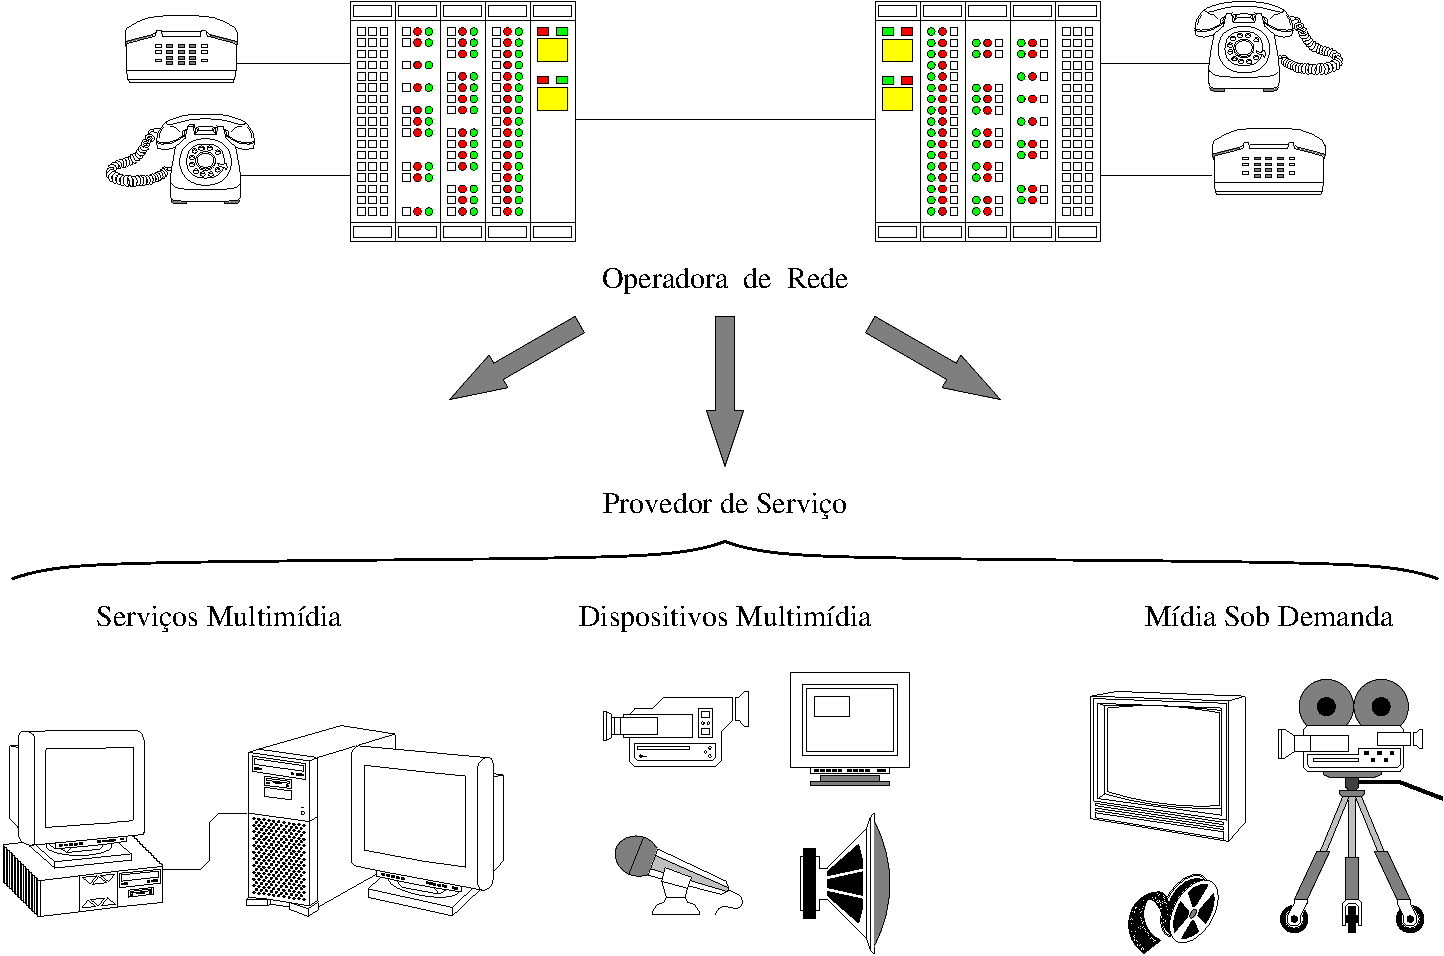
\includegraphics[width=\textwidth]{./CapituloExemplo/figura1}%% Dimensões e localização
%\fonte{\citet{Larsson2003}.}%% Fonte (quando criado pelo autor, usar Autoria Própria)
%\end{figure}

%% Classe e opções de documento
\documentclass[%% Opções
%% -- Opções da classe MEMOIR --
  12pt,%% Tamanho da fonte: 10pt, 11pt, 12pt, etc.
  a4paper,%% Tamanho do papel: a4paper (A4), letterpaper (carta), etc.
  % fleqn,%% Alinhamento das equações à esquerda (comente para alinhamento centralizado)
  % leqno,%% Numeração das equações no lado esquerdo (comente para lado direito)
  oneside,%% IMPRESSÃO dos elementos textuais e pós-textuais: oneside (apenas no anverso) ou twoside (anverso e verso, se mais de 100 p.) (insere páginas em branco).
%%  
%% -- Opções da classe ABNTEX2 --
  sumario = abnt-6027-2012,%% Formatação do sumário: tradicional (estilo tradicional) ou abnt-6027-2012 (norma ABNT 6027-2012)
  chapter = TITLE,%% Títulos de capítulos em maiúsculas (comente para desabilitar)
  section = TITLE,%% Títulos de seções secundárias em maiúsculas (comente para desabilitar)
  % subsection = TITLE,%% Títulos de seções terciárias em maiúsculas (comente para desabilitar)
  % subsubsection = TITLE,%% Títulos de seções quartenárias em maiúsculas (comente para desabilitar)
%%  
%% -- Opções da classe UTFPRCT-TEX --
  pretextualoneside,%% Impressão dos elementos pré-textuais: pretextualoneside (anverso) ou pretextualtwoside (anverso e verso)
  fontetimes,%% Fonte do texto: fontetimes (times), fontearial (arial) ou fontecourier (courier), fontemodern (lmodern - default latex). Times and Arial are ABNT recommended
   %vinculoscoloridos,%% Cores nos vínculos (citações, arquivos, links, url, etc.) (comente para desabilitar). NBR 14724/2011: cor preta (inclusive hyperlinks)
  semrecuonosumario,%% Remoção do recuo dos itens no sumário (comente para adição do recuo, se estilo tradicional)
  %inserirbackref,%% Inserir backref na lista de referências (e.g., Citado na página...)
  usemakeindex,%% Compilação de glossários e índices utilizando makeindex (comente para desabilitar)
  legendascentralizadas,%% Alinhamento das legendas centralizado (comente para alinhamento à esquerda)
%%  
%% -- Opções da folha de aprovação -- 
%% O mais comum é anexar o PDF do termo de aprovação sem assinaturas. As opções abaixo são para o formato da pós-graduação UTFPR-PG (Ponta Grossa) e podem servir de placeholder para este template.
  %aprovacaoestiloppg,%% Folha de aprovação do programa de pós-graduação no estilo do PPG (comente para estilo padrão)
  %pardeassinaturas,%% Assinaturas na folha de aprovação em até duas colunas (comente para em uma única coluna)
  % linhasdeassinaturas,%% Linhas de assinaturas na folha de aprovação (comente para remover as linhas)
%%  
%% -- Opções do pacote babel (hifenização) -- % 
  %french,%% Idioma adicional para hifenização (suporte parcial)
  %spanish,%% Idioma adicional para hifenização (suporte parcial)
  english,%% Idioma adicional para hifenização  (colocar em último para doc. em inglês)  
  brazil%% Idioma principal do documento (último da lista) 
]{utfprct}%% Classe utfprct

%%%%%%%%
% Documento em Inglês: colocar o "english" como último idioma carregado no documentclass, sendo o último a língua principal do documento.
%%%%%%%%

%%%%%%%%
%% Configuração dos avisos (warnings)
%% Comportamento do Tex quando um PDF é incluído e possui uma versão mais nova que a versão mínima especificada em \pdfminorversion. Opções: -1 (no info), 0 (default, warning), 1 (error)
\pdfinclusionerrorlevel=-1%no warning 
%\pdfminorversion=5%pdf minor output version (default 5)

%% [Badbox] Underfull e Overfull nível de aviso (filtra o que está abaixo)
\hbadness=5000%0 até 10000 (max) nível de badness
\vbadness=1000%0 até 10000 (max) nível de badness
%\hfuzz=0.01pt%excesso permitido de largura (\hbox)para ser considerado overfull
%\vfuzz=0.001pt%excesso permitido de altura (\vbox) para ser considerado overfull
%\overfullrule=10mm%adicionar aviso visual para um badbox
%%%%%%%%

%%%%%%%%
%% Pacotes carregados nas classes:
%%   memoir: abstract, appendix, array, booktabs, ccaption, chngcntr, chngpage, dcolumn, delarray, enumerate, epigraph, framed, ifmtarg, ifpdf, index, makeidx, moreverb, needspace, newfile, nextpage, parskip, patchcmd, setspace, shortvrb, showidx, tabularx, titleref, titling, tocbibind, tocloft, verbatim, verse.
%%   memoir (similares): crop, fancyhdr, geometry, sidecap, subfigure, titlesec.
%%   abntex2: babel, bookmark, calc, enumitem, ifthen, hyperref, textcase.
%%   utfprct: abntex2cite, ae, algorithmic, amsmath, backref, breakurl, caption, subcaption, cmap, color, eepic, epic, epsfig, etoolbox, fancyhdr, fix-cm, fontenc, glossaries, graphics, graphicx, helvet, hyphenat, indentfirst, inputenc, lastpage, morewrites, nomencl, sfmath, sistyle, substr, times, xtab, pdfpages.

%% Pacotes adicionais (\usepackage[options]{package})
\usepackage{bigdelim, booktabs, colortbl, longtable, multirow}%% Ferramentas para tabelas
\usepackage{amssymb, amstext, amsthm, icomma}%% Ferramentas para linguagem matemática
\usepackage{pifont, textcomp, wasysym}%% Símbolos de texto

% Refinamento tipográfico: diminui badboxes
\usepackage{microtype}%

%% Comandos personalizados (\newcommand{name}[num]{definition})
\newcommand{\cpp}{\texttt{C$++$}}%% C++
\newcommand{\latex}{\LaTeX}%% LaTeX
\newcommand{\ds}{\displaystyle}%% Tamanho normal das equações
\newcommand{\bsym}[1]{\boldsymbol{#1}}%% Texto no modo matemático em negrito
\newcommand{\mr}[1]{\mathrm{#1}}%% Texto no modo matemático normal (não itálico)
\newcommand{\der}{\mr{d}}%% Operador diferencial
\newcommand{\deri}[2]{\frac{\der#1}{\der#2}}%% Derivada ordinária
\newcommand{\derip}[2]{\frac{\partial#1}{\partial#2}}%% Derivada parcial
\newcommand{\pare}[1]{\left(#1\right)}%% Parênteses
\newcommand{\colc}[1]{\left[#1\right]}%% Colchetes
\newcommand{\chav}[1]{\left\lbrace#1\right\rbrace}%% Chaves
\newcommand{\sen}{\operatorname{sen}}%% Operador seno
\newcommand{\senh}{\operatorname{senh}}%% Operador seno hiperbólico
\newcommand{\tg}{\operatorname{tg}}%% Operador tangente
\newcommand{\tgh}{\operatorname{tgh}}%% Operador tangente hiperbólico  
\ifthenelse{\equal{\languagename}{english}}{%%
\newcommand{\nomeequacao}{Equation}
\newcommand{\nomeequacoes}{Equations}
}{%default pt
\newcommand{\nomeequacao}{Equação}
\newcommand{\nomeequacoes}{Equações}
}%  
\newcommand{\seqref}[1]{\nomeequacao~\eqref{#1}}%% Referência de uma única equação
\newcommand{\meqref}[1]{\nomeequacoes~\eqref{#1}}%% Referência de multiplas equações
\newcommand{\citep}[1]{\cite{#1}}%% Atalho para citação implícita
\newcommand{\citet}[1]{\citeonline{#1}}%% Atalho para citação explícita
\newcommand{\citepa}[1]{(\citeauthor{#1})}%% Atalho para citação implícita (somente autor)
\newcommand{\citeta}[1]{\citeauthoronline{#1}}%% Atalho para citação explícita (somente autor)
\newcommand{\citepy}[1]{(\citeyear{#1})}%% Atalho para citação implícita (somente ano)
\newcommand{\citety}[1]{\citeyear{#1}}%% Atalho para citação explícita (somente ano)

%allow fixed size on collums with text position
\newcolumntype{L}[1]{>{\raggedright\let\newline\\\arraybackslash\hspace{0pt}}m{#1}}
\newcolumntype{C}[1]{>{\centering\let\newline\\\arraybackslash\hspace{0pt}}m{#1}}
\newcolumntype{R}[1]{>{\raggedleft\let\newline\\\arraybackslash\hspace{0pt}}m{#1}}

%%%%%%%%%%%%%%%%%%%%%%%%%%%%%%%%%%%%%%%%%%%%%%%
%%%%%%%%%%%%%%%%%%%%%%%%%%%%%%%%%%%%%%%%%%%%%%%
%% Configuração das entradas
%%

%% Arquivo de dados do modelo de documento LaTeX para produção de trabalhos acadêmicos da UTFPR
%% UTFPRCT-TEX, v1.0.6 wmeira on 2021/10/11
%% Copyright (C) 2020- by William H. T. Meira
%%
%% Modified version of project 'utfprpgtex' maintained 
%% by Luiz E. M. Lima
%%
%% This work may be distributed and/or modified under the
%% conditions of the LaTeX Project Public License, either version 1.3
%% of this license or (at your option) any later version.
%% The latest version of this license is in
%%   http://www.latex-project.org/lppl.txt
%% and version 1.3 or later is part of all distributions of LaTeX
%% version 2005/12/01 or later.
%%
%% This work has the LPPL maintenance status `maintained'.
%%
%% The Current Maintainer of this work is William H. T. Meira.
%%
%% This project consists mainly of files: 'utfprct.cls', 'utfprct.tex', 
%% 'utfprct-dados.tex' 
%% 
%% The 'abntex2-alf.bst' and 'abntex2-num.bst' files are slightly
%% modified versions of the bibtex styles from abntex2 (v.1.9.7)
%% package to suit NBR6023/2018 (not yet implemented there). 
%% Complementary, 'abntex2-alf-en.bst' and 'abntex2-num-en.bst' are
%% english versions of the respective bibtex styles.
%%
%% Contribute to improve this project (github repo):
%% https://github.com/wmeira/utfprct-tex

%%%%%%%%%%%%%%%%%%%%%%%%%%%%%%%%%%%%%%%%%%%%%%%
%%%%%%%%%%%%%%%%%%%%%%%%%%%%%%%%%%%%%%%%%%%%%%%
%% Tutorial do Documento de Dados 
%%%%%%%%%%%%%%%%%%%%%%%%%%%%%%%%%%%%%%%%%%%%%%%
%%
%% O 'utfprct-dados.tex' contém todos as informações do documento, 
%% metadados e outros valores importantes para o preenchimento dos 
%% elementos pré-textuais: capa, folha de rosto, resumo, abstract.
%% 
%% Não é necessário preencher todos os campos, existem campos mais
%% específicos para o tipo de documento sendo elaborado. Quando TCC,
%% por exemplo, não é necessário definir dados do programa de 
%% pós-graduação. Todos os dados inseridos estarão disponíveis para
%% inserção no tex usando o padrão '\imprimir + nomedodadominusculo'. 
%% Por exemplo, para imprimir o tipo do documento ('\TipoDeDocumento'),
%% usar '\imprimirtipodedocumento'.
%%
%% É possível customizar a descrição do documento na folha de rosto. 
%% Exemplos de descrição são fornecidos para guiar a escrita do texto,
%% em que pode-se utilizar os dados já definidos com o padrão descrito.
%%
%% Existe a possibilidade de inserir dados de uma instituição de 
%% cotutela quando se aplicar. 
%%
%% Os dados da ficha catalográfica são fornecidos pela biblioteca
%% e, na maioria das vezes, apenas anexa-se a folha digitalizada
%% na região definida dos elementos pré-textuais.
%%
%% A folha de aprovação é, na maioria das vezes, fornecido 
%% digitalmente pelo departamento ou pelo orientador após a defesa e 
%% deverá ser anexada ao documento na região definida dos elementos 
%% pré-textuais. Recomenda-se apenas anexar a folha de aprovação sem
%% precisar alterar os dados específicos aqui presentes, pois foram
%% criados originalmente para o template da folha de aprovação da
%% UTFPR-PG, presente no projeto base, e foram apenas mantidos.
%%
%%%%%%%%%%%%%%%%%%%%%%%%%%%%%%%%%%%%%%%%%%%%%%%
%%%%%%%%%%%%%%%%%%%%%%%%%%%%%%%%%%%%%%%%%%%%%%%

%%%%%%%%%%%%%%%%%%%%%%%%%%%%%%%%%%%%%%%%%%%%%%%
%% Informações do Documento
%%%%%%%%%%%%%%%%%%%%%%%%%%%%%%%%%%%%%%%%%%%%%%%

%% Tipo de documento (opções: "Tese", "Dissertação", "Trabalho de Conclusão de Curso"
\TipoDeDocumento{Trabalho de Conclusão de Curso}%copiar exatamente uma das opções 

%% [abstract] Document type: "Thesis", "Dissertation", "Bachelor Thesis"
\DocumentType{Bachelor Thesis}%

%% Nível de formação: "Doutorado", "Mestrado", "Bacharelado"
\NivelDeFormacao{Bacharelado}%

%% [abstract] Formation level: "Doctorate", "PhD", "Master's Degree", "Bachelor's Degree"
\FormationLevel{Bachelor's Degree}%

%% Título ou grau pretendido: "Doutor", "Mestre" ou "Bacharel"
\TituloPretendido{Bacharel}%

%%%%%%%%%%%%%%%%%%%%%%%%%
%% Por padrão, o título principal será o \TituloDoDocumento (português)
%% Se a língua do documento for definida como inglês, será o \DocumentTitle

%% Título do documento em PORTUGUÊS (resumo)
\TituloDoDocumento{%%
Desenvolvimento de um multímetro de três canais com comunicação sem fio de baixo custo para laboratórios da Universidade Tecnológica Federal do Paraná
}%

%% Título do trabalho em INGLÊS (abstract)
\DocumentTitle{%%
Development of a low cost three-channel multimeter with wireless communication for laboratories at the Federal Technological University of Paraná
}%

%% Título em múltiplas linhas na capa, folha de rosto e termo de aprovação
%% Use o comando \par para indicar a quebra de linha
%%
%% A CAPA apresentará o título no formato de múltiplas linhas
%% para a respectiva língua do documento definida.
%%
%% Na folha de rosto, caso a língua do documento não seja português, aparecerá o
%% \TituloEmMultiplasLinhasIngles seguido pela tradução \TituloEmMultiplasLinhas
%%
\TituloEmMultiplasLinhas{%%
Desenvolvimento de um multímetro de três canais com comunicação sem fio\par 
de baixo custo para laboratórios da Universidade Tecnológica Federal do Paraná
}%

\TituloEmMultiplasLinhasIngles{%%
Development of a low cost three-channel multimeter with\par
wireless communication for laboratories at the Federal Technological University of Paraná
}%

%%%%%%%%%%%%%%%%%%%%%%%%%


%% Data da defesa
\Dia{05}%% Dia (opcional: usado na ficha catalográfica apenas)
\MesPorExtenso{junho}%% mês por extenso (opcional: usado na ficha catalográfica apenas)
\Ano{2023}%% Ano

%% Palavras-chave e keywords (máximo 5)
\NumeroDePalavrasChave{5}%% Número de palavras-chave 
\PalavraChaveA{multímetro}%% Palavra-chave A
\PalavraChaveB{wifi}%% Palavra-chave B
\PalavraChaveC{laboratório}%% Palavra-chave C
\PalavraChaveD{baixo-custo}%% Palavra-chave D
\PalavraChaveE{ondas}%% Palavra-chave E

\NumeroDeKeywords{\imprimirnumerodepalavraschave}%% Número de keywords (mesmo que palavras-chave)
\KeywordA{multimeter}%% Keyword A
\KeywordB{wireless}%% Keyword B
\KeywordC{lab}%% Keyword C
\KeywordD{low-cost}%% Keyword D
\KeywordE{waves}%% Keyword E

%%%%%%%%%%%%%%%%%%%%%%%%%%%%%%%%%%%%%%%%%%%%%%%
%% Informação do Autor(a) ou Autores(as) (TCC)
%%%%%%%%%%%%%%%%%%%%%%%%%%%%%%%%%%%%%%%%%%%%%%%

%%% Autor(a)
%% Usado para citação: "\SobrenomeDoAutor, PrenomeDoAutor" (ex: "Doe, John" ou "Doe, J.")
\NomeDoAutor{Andrey Alexandre Guimarães}%% Nome completo do(a) autor(a)
\SobrenomeDoAutor{Guimarães}%% Último nome do(a) autor(a)
\PrenomeDoAutor{Andrey A.}%% Nome do(a) autor(a) sem último nome

%%% Autor(a) 2 (opcional)
%% *Considera apenas se "\TipoDeDocumento" == "Trabalho de Conclusão de Curso"
\AtribuiAutorDois{true}%% Insere ou remove autor(a) 2: "true" ou "false"
\NomeDoAutorDois{Rafael Felipe Parolin}%% Nome completo do(a) autor(a) 2
\SobrenomeDoAutorDois{Parolin}%% Último nome do(a) autor(a) 2
\PrenomeDoAutorDois{Rafael F.}%% Nome do(a) autor(a) 2 sem último nome

%%% Autor(a) 3 (opcional)
%% *Considera apenas se "\TipoDeDocumento" == "Trabalho de Conclusão de Curso"
\AtribuiAutorTres{false}%% Insere ou remove autor(a) 3: "true" ou "false"
\NomeDoAutorTres{Nome do(a) Autor(a) 3}%% Nome completo do(a) autor(a) 3
\SobrenomeDoAutorTres{Último Nome}%% Último nome do(a) autor(a) 3
\PrenomeDoAutorTres{Nome do(a) Autor(a) 3 Sem Último}%% Nome do(a) autor(a) 3 sem último nome

%%%%%%%%%%%%%%%%%%%%%%%%%%%%%%%%%%%%%%%%%%%%%%%%%%
%% Informações do Orientador(a) e Coorientador(a)
%%%%%%%%%%%%%%%%%%%%%%%%%%%%%%%%%%%%%%%%%%%%%%%%%%

%% Orientador(a)
%% Usado para citação: "\SobrenomeDoOrientador, PrenomeDoOrientador" (ex: "Doe, John" ou "Doe, J.")
\AtribuicaoOrientador{Orientador(a)}%% Atribuição "Orientador(a)"
\TituloDoOrientador{Prof. Dr.}%% Título do(a) orientador(a)
\NomeDoOrientador{Juan Camilo Castellanos Rodriguez}%% Nome completo do(a) orientador(a)
\SobrenomeDoOrienador{Rodriguez}%% Último nome do(a) orientador(a)
\PrenomeDoOrientador{Juan C. C.}%% Nome do(a) orientador(a) sem último nome

%% Coorientador(a) (opcional)
%% Usado para citação: "\SobrenomeDoCoorientador, PrenomeDoCoorientador" (ex: "Doe, John" ou "Doe, J.")
\AtribuiCoorientador{false}%% Insere ou remove o(a) coorientador(a): "true" ou "false"
\AtribuicaoCoorientador{Coorientador(a)}%% Atribuição "Coorientador(a)"
\TituloDoCoorientador{Prof(a). Dr(a).}%% Título do(a) coorientador(a)
\NomeDoCoorientador{Nome Completo do(a) Coorientador(a)}%% Nome completo do(a) coorientador(a)
\SobrenomeDoCoorienador{Último Nome}%% Último nome do(a) coorientador(a)
\PrenomeDoCoorientador{Nome do(a) Coorientador(a) Sem Último}%% Nome do(a) coorientador(a) sem último nome

%%%%%%%%%%%%%%%%%%%%%%%%%%%%%%%%%%%%%%%%%%%%%%%%%%
%% Informações da Instituição
%%%%%%%%%%%%%%%%%%%%%%%%%%%%%%%%%%%%%%%%%%%%%%%%%%

%% Nome da instituição
\Instituicao{Universidade Tecnológica Federal do Paraná}

%% [abstract] Institution name (*nome sem traduzir é o recomendado para docs. da UTFPR)
\Institution{Universidade Tecnológica Federal do Paraná}

%% Sigla da Instituição
\SiglaInstituicao{UTFPR}

%% Nome da cidade (câmpus)
\Cidade{Curitiba}

%% Diretoria: "Graduação e Educação Profissional" ou "Pesquisa e Pós-Graduação" (opcional)
\Diretoria{Graduação e Educação Profissional}

%% Nome do departamento ou da coordenação (opcional: mais comum no Bacharelado: Departamento de Informática)
\Departamento{Departamento Acadêmico de Eletrotécnica}

%% Sigla do departamento (opcional, ex: DAINF, DAMEC, DAMAT...)
\SiglaDepartamento{DAELT}

%% Nome do curso bachalerado ou pós-graduação (PPG) (ex: "Engenharia de Computação",  "Engenharia El{\'e}trica e Inform{\'a}tica Industrial") 
\Curso{Engenharia Elétrica}

%% [abstract] Course name
\Course{Electrical Engineering}

%% Programa ou nome do curso completo (capa)
%% "Bachalerado em Engenharia de Computação"
%% "Programa de Pós-Graduação em Engenharia Elétrica e Informática Industrial"
\Programa{Bachalerado em \imprimircurso}

%% Sigla do programa de pós-graduação (opcional, ex: CPGEI, PPGCA)
\SiglaDoPPG{PPG}

%% Nome da área de concentração
\AreaDeConcentracao{Nome da Área de Concentração}

%%%%%%%%%%%%%%%%%%%%%%%%%%%%%%%%%%%%%%%%%%%%%%%%%%%%%%
%% Informações de Cotutela (Duplo Grau) (opcional)
%%%%%%%%%%%%%%%%%%%%%%%%%%%%%%%%%%%%%%%%%%%%%%%%%%%%%%

%% Insere dados de cotutela: "true" ou "false"
\AtribuiCotutela{false}

%% Nome da instituição de cotutela
\InstituicaoCotutela{Universidade Da Cotutela}

%% [abstract] Institution name
\InstitutionCotutela{Double Degree University}

%% Sigla da instituição de cotutela
\SiglaInstituicaoCotutela{UC}

%% Nome do departamento ou da coordenação da inst. de cotutela (mais comum no Bacharelado: Departamento de Informática)
\DepartamentoCotutela{Nome do Departamento ou da Coordenação}

%% Sigla do departamento da inst. cotutela (ex: DAINF, DAMEC, DAMAT...)
\SiglaDepartamentoCotutela{DPT-EXT}

%% Nome do curso bachalerado ou pós-graduação (PPG) na instituição de cotutela (ex: "Engenharia de Computação",  "Engenharia El{\'e}trica e Inform{\'a}tica Industrial")
\CursoCotutela{Nome do Curso Cotutela}

%% [abstract] Course name 
\CourseCotutela{Second Degree Course}

%% Programa ou nome do curso completo na inst. cotutela (capa)
%% "Bachalerado em Engenharia de Computação"
%% "Programa de Pós-Graduação em Engenharia Elétrica e Informática Industrial"
\ProgramaCotutela{Programa de Doutoral em \imprimircursocotutela}

%% Sigla do programa externo de pós-graduação
\SiglaDoPPGCotutela{PPG-EXT}

%% Nome da área de concentração na instituição de cotutela
\AreaDeConcentracaoCotutela{Nome da Área de Concentração}

%% Nível de formação que será fornecido na referência do doc.
\NivelDeFormacaoResumo{Duplo doutorado}
\FormationLevelAbstract{Double PhD}

%% Informacoes do orientador(a) na instituição de cotutela

%% Orientador(a) da instituição de cotutela
%% Usado para citação: "\SobrenomeDoOrientador, PrenomeDoOrientador" (ex: "Doe, John" ou "Doe, J.")
\AtribuicaoOrientadorCotutela{Orientador(a)}%% Atribuição "Orientador(a)"
\TituloDoOrientadorCotutela{Prof(a). Dr(a).}%% Título do(a) orientador(a)
\NomeDoOrientadorCotutela{Nome Completo do(a) Orientador(a)}%% Nome completo do(a) orientador(a)
\SobrenomeDoOrienadorCotutela{Último Nome}%% Último nome do(a) orientador(a)
\PrenomeDoOrientadorCotutela{Nome do(a) Orientador(a) Sem Último}%% Nome do(a) orientador(a) sem último nome

%% Coorientador(a) da instituição de cotutela
%% Usado para citação: "\SobrenomeDoCoorientador, PrenomeDoCoorientador" (ex: "Doe, John" ou "Doe, J.")
\AtribuiCoorientadorCotutela{false}%% Insere ou remove o(a) coorientador(a) da cotutela: "true" ou "false"
\AtribuicaoCoorientadorCotutela{Coorientador(a)}%% Atribuição "Coorientador(a)"
\TituloDoCoorientadorCotutela{Prof(a). Dr(a).}%% Título do(a) coorientador(a)
\NomeDoCoorientadorCotutela{Nome Completo do(a) Coorientador(a)}%% Nome completo do(a) coorientador(a)
\SobrenomeDoCoorienadorCotutela{Último Nome}%% Último nome do(a) coorientador(a)
\PrenomeDoCoorientadorCotutela{Nome do(a) Coorientador(a) Sem Último}%% Nome do(a) coorientador(a) sem último nome

%%%%%%%%%%%%%%%%%%%%%%%%%%%%%%%%%%%%%%%%%%%%%%%%%%
%% Folha de Rosto
%%%%%%%%%%%%%%%%%%%%%%%%%%%%%%%%%%%%%%%%%%%%%%%%%%

%% Se desejar usar os dados inseridos, eles estão disponíves
%% usando o padrão '\imprimir + nomedodadominusculo'. Por exemplo,
%% para imprimir o tipo do documento ('\TipoDeDocumento'), usar
%% '\imprimirtipodedocumento'

%% Descrição do documento na folha de rosto (exemplos)
\DescricaoDoDocumento{
\imprimirtipodedocumento\ apresentado(a) como requisito para obtenção do título(grau) de \imprimirtitulopretendido\ em \imprimircurso, do \imprimirppgoudepartamento, da \imprimirinstituicao\ (\imprimirsiglainstituicao).
}

% Exemplo: Mestrado
%\DescricaoDoDocumento{
%\imprimirtipodedocumento\ apresentada como requisito para obtenção do grau de \imprimirtitulopretendido\ em \imprimircurso\ da \imprimirinstituicao\ (\imprimirsiglainstituicao).
%}

% Exemplo: Doutorado
%\DescricaoDoDocumento{
%\imprimirtipodedocumento\ apresentada como requisito para obtenção do título de \imprimirtitulopretendido\ em \imprimircurso\ da \imprimirinstituicao\ (\imprimirsiglainstituicao).
%}


%% Insere ou remove descrição da cotutela (extra) na folha de rosto: "true" ou "false". 
%% Se "true", a descrição do documento será colocada na folha de rosto, logo abaixo do orientador(a) e coorientador(a) da primeira inst. e depois o orientador(a) e coorientador(a) da inst. de cotutela. 
%% Se "false", os nomes do orientador(a) e coorientador(a) aparecerão logo abaixo do orientador(a) da primeira instituição, sem uma descrição extra. Neste caso, recomenda-se revisar a "\DescricaoDoDocumento" para contemplar ambas as instituições.   
\AtribuiDescricaoCotutela{false}

%% Segunda Descricao da Inst. de Cotutela na folha de rosto (exemplos)
\DescricaoDoDocumentoCotutela{
\imprimirtipodedocumento\ apresentado(a) como requisito à obtenção do título de \imprimirtitulopretendido\ em \imprimircursocotutela, do \imprimirppgoudepartamentocotutela, da \imprimirinstituicaocotutela.  
%\imprimirtipodedocumento\ apresentada à Comissão de Acompanhamento de Tese do Programa Doutoral em \imprimircursocotutela\ do \imprimirinstituicaocotutela\ (\imprimirsiglainstituicaocotutela) como requisito à obtenção de grau de \imprimirtitulopretendido\ na área de concentração \imprimirareadeconcentracaocotutela.
}

%%%%%%%%%%%%%%%%%%%%%%%%%%%%%%%%%%%%%%%%%%%%%%%%%%
%% Ficha Catalográfica* (opcional)
%%%%%%%%%%%%%%%%%%%%%%%%%%%%%%%%%%%%%%%%%%%%%%%%%%

%% *Pode ser usado como placeholder, porém para entrega deve-se inserir a ficha catolográfica digitalizado (PDF) pela biblioteca da UTFPR.

\NumeroDaPublicacao{00/\imprimirano}%% Número da publicação - Fornecido pela biblioteca
\CDDOuCDU{CDD 000.00}%% Classificação Decimal Dewey (CDD) ou Classificação Decimal Universal (CDU) - Fornecida pela biblioteca

\TituloDaFichaCatalografica{%% Título da ficha catalográfica
  Ficha catalográfica elaborada pelo Departamento de Biblioteca da \par \imprimirinstituicao, Câmpus \imprimircidade \par n.
  \imprimirnumerodapublicacao
}

%%%%%%%%%%%%%%%%%%%%%%%%%%%%%%%%%%%%%%%%%%%%%%%%%%
%% Folha de aprovação (Formato UTFPR-PG)* (opcional)
%%%%%%%%%%%%%%%%%%%%%%%%%%%%%%%%%%%%%%%%%%%%%%%%%%

%% *Pode ser usado como placeholder, porém para entrega final prefere-se a folha (termo) de aprovação digitalizado (PDF) fornecido pelo departamento ou orientador.

\NumeroDaTeseOuDissertacao{00/\imprimirano}%% Número da Tese ou Dissertação - Fornecido pelo programa de pós-graduação
\NumeroDaFichaCatalografica{A000}%% Número da ficha catalográfica - Fornecido pela biblioteca

\TituloDoResponsavelTCC{Prof(a). Dr(a).}%% Título do(a) responsável pelos TCC
\NomeDoResponsavelTCC{Nome do(a) Responsável}%% Nome completo do(a) responsável pelos TCC
\AtribuicaoCoordenador{Coordenador(a)}%% Atribuição "Coordenador(a)" do curso
\TituloDoCoordenador{Prof(a). Dr(a).}%% Título do(a) coordenador(a) do curso
\NomeDoCoordenador{Nome do(a) Coordenador(a)}%% Nome completo do(a) coordenador(a) do curso

\TextoDeAprovacao{%% Texto de aprovação
  %% Exemplo de texto de aprovação para Tese ou Dissertação (descomente a próxima linha para utilizá-lo):
  Esta \imprimirtipodedocumento\ foi apresentada às 00:00 de \imprimirdia\ de \imprimirmesporextenso\ de \imprimirano\ como requisito parcial para a obtenção do título de \imprimirtitulopretendido\ em \imprimircurso, na área de concentração em \imprimirareadeconcentracao\ e na linha de pesquisa em (Nome da Linha de Pesquisa), do Programa de Pós-Graduação em \imprimircurso. O(A) candidato(a) foi arguido(a) pela Banca Examinadora composta pelos professores abaixo citados. Após deliberação, a Banca Examinadora considerou o trabalho aprovado.
  %% Exemplo de texto de aprovação para Trabalho de Conclusão de Curso (descomente a próxima linha para utilizá-lo):
  % Este \imprimirtipodedocumento\ foi apresentado em \imprimirdia\ de \imprimirmesporextenso\ de \imprimirano\ como requisito parcial para a obtenção do título de \imprimirtitulopretendido\ em \imprimircurso. O(A) candidato(a) foi arguido(a) pela Banca Examinadora composta pelos professores abaixo assinados. Após deliberação, a Banca Examinadora considerou o trabalho aprovado.
}

\AvisoDeAprovacao{%% Aviso de aprovação
  %% Exemplo de aviso de aprovação para Tese ou Dissertação (descomente a próxima linha para utilizá-lo):
  A Folha de Aprovação assinada encontra-se no \par Departamento de Registros Acadêmicos da UTFPR -- Câmpus \imprimircidade
  %% Exemplo de aviso de aprovação para Trabalho de Conclusão de Curso (descomente a próxima linha para utilizá-lo):
  % -- O Termo de Aprovação assinado encontra-se na Coordenação do Curso --
}

%% Banca examinadora: 3 membros (Trabalho de Conclusão de Curso ou Dissertação); 5 a 7 membros (Tese)
\MembroAIgualOrientador{true}%% Insere ou remove o membro A igual ao(à) orientador(a): "true" ou "false"
\MembroA{Nome do Membro A}%% Nome completo do membro A - Presidente (automático se orientador(a))
\TituloDoMembroA{Prof(a). Dr(a).}%% Título do membro A - Presidente (automático se orientador(a))
\InstituicaoDoMembroA{Instituição do Membro A}%% Nome da instituição do membro A - Presidente (automático se orientador(a))
\MembroB{Nome do Membro B}%% Nome completo do membro B
\TituloDoMembroB{Prof(a). Dr(a).}%% Título do membro B
\InstituicaoDoMembroB{Instituição do Membro B}%% Nome da instituição do membro B
\MembroC{Nome do Membro C}%% Nome completo do membro C
\TituloDoMembroC{Prof(a). Dr(a).}%% Título do membro C
\InstituicaoDoMembroC{Instituição do Membro C}%% Nome da instituição do membro C
\MembroD{Nome do Membro D}%% Nome completo do membro D
\TituloDoMembroD{Prof(a). Dr(a).}%% Título do membro D
\InstituicaoDoMembroD{Instituição do Membro D}%% Nome da instituição do membro D
\MembroE{Nome do Membro E}%% Nome completo do membro E
\TituloDoMembroE{Prof(a). Dr(a).}%% Título do membro E
\InstituicaoDoMembroE{Instituição do Membro E}%% Nome da instituição do membro E
\AtribuiMembroF{false}%% Insere ou remove o Membro F: "true" ou "false"
\MembroF{Nome do Membro F}%% Nome completo do membro F
\TituloDoMembroF{Prof(a). Dr(a).}%% Título do membro F
\InstituicaoDoMembroF{Instituição do Membro F}%% Nome da instituição do membro F
\AtribuiMembroG{false}%% Insere ou remove o Membro G: "true" ou "false"
\MembroG{Nome do Membro G}%% Nome completo do membro G
\TituloDoMembroG{Prof(a). Dr(a).}%% Título do membro G
\InstituicaoDoMembroG{Instituição do Membro G}%% Nome da instituição do membro G%% Realize as modificações pertinentes no arquivo "utfprct-dados.tex"

%% Ferramenta para criação de índices
\makeindex%% Não comente esta linha

%% Ferramenta para criação de glossários
\makeglossaries%% Não comente esta linha

%% Entradas da lista de abreviaturas, siglas e acrônimos
%%%% LISTA DE ABREVIATURAS, SIGLAS E ACRÔNIMOS
%%
%% Relação, em ordem alfabética, das abreviaturas (representação de uma palavra por meio de alguma(s) de sua(s) sílaba(s) ou
%% letra(s)), siglas (conjunto de letras iniciais dos vocábulos e/ou números que representa um determinado nome) e acrônimos
%% (conjunto de letras iniciais dos vocábulos e/ou números que representa um determinado nome, formando uma palavra pronunciável).
%%
%%
%% Este arquivo para definição de abreviaturas, siglas e acrônimos é utilizado com a opção \incluirlistadeacronimos{glossaries}
%%
%% Vantagens do modo com "glossaries" em relação ao modo "file":
%%   1) Ordena automaticamente a lista
%%	 2) Apenas os termos referenciados são colocados na lista


%% Como referenciar: 
%% \gls{lp} = Linear Programming (LP)  (First use)
%% \gls{lp} = LP (Next uses)
%% \glspl{lp} = LPs
%% \glsentrytext{lp} = Linear Programming    (recommended for chapter/section/....)
%% \glsentrylong{lp} = Linear Programming
%% \glsentryshort{lp} = LP

%% Para acrônimos também funciona:  
%% \acrlong{lp} = Linear Programming
%% \acrshort{lp} = LP

%% Abreviaturas: \abreviatura{rótulo}{representação}{definição}

\abreviatura{art.}{art.}{Artigo}
\abreviatura{cap.}{cap.}{Capítulo}
\abreviatura{sec.}{sec.}{Seção}

%% Siglas: \sigla{rótulo}{representação}{definição}

\sigla{abnt}{ABNT}{Associação Brasileira de Normas Técnicas}
\sigla{cnpq}{CNPq}{Conselho Nacional de Desenvolvimento Científico e Tecnológico}
\sigla{eps}{EPS}{\textit{Encapsulated PostScript}}
\sigla{pdf}{PDF}{Formato de Documento Portátil, do inglês \textit{Portable Document Format}}
\sigla{ps}{PS}{\textit{PostScript}}
\sigla{utfpr}{UTFPR}{Universidade Tecnológica Federal do Paraná}

%% Acrônimos: \acronimo{rótulo}{representação}{definição}

\acronimo{gimp}{Gimp}{Programa de Manipulação de Imagem GNU, do inglês \textit{GNU Image Manipulation Program}}
\acronimo{tcc}{TCC}{Trabalho de Conclusão de Curso}% Comente para remover este item

%% Entradas do glossário
%%%% GLOSSÁRIO
%%
%% Relação de palavras ou expressões técnicas de uso restrito ou de sentido obscuro, utilizadas no texto, acompanhadas das
%% respectivas definições.

%% Entradas do glossário: \newglossaryentry{rótulo}{informações da entrada}

\newglossaryentry{pai}{%% Informações da entrada
    name        = {pai},
    plural      = {pais},
    description = {um exemplo de entrada pai que possui subentradas (entradas filhas)}
}

\newglossaryentry{componente}{%% Informações da entrada
    name        = {componente},
    plural      = {componentes},
    parent      = {pai},
    description = {um exemplo de uma entrada componente, subentrada da entrada chamada \gls{pai}}
}

\newglossaryentry{filho}{%% Informações da entrada
    name        = {filho},
    plural      = {filhos},
    parent      = {pai},
    description = {um exemplo de uma entrada filha (subentrada) da entrada chamada \gls{pai}. Trata-se de uma entrada irmã da entrada chamada \gls{componente}}
}

\newglossaryentry{equilibrio}{%% Informações da entrada
    name        = {equilíbrio da configuração},
    see         = [veja também]{componente},
    description = {uma consistência entre os \glspl{componente}}
}

\newglossaryentry{tex}{%% Informações da entrada
    name        = {\TeX},
    sort        = {TeX},
    description = {é um sistema de tipografia criado por Donald E. Knuth}
}

\newglossaryentry{latex}{%% Informações da entrada
    name        = {\latex},
    sort        = {LaTeX},
    description = {um conjunto de macros para o processador de textos \gls{tex}, utilizado amplamente para a produção de textos matemáticos e científicos devido à sua alta qualidade tipográfica}
}

\newglossaryentry{bibtex}{%% Informações da entrada
    name        = {Bib\TeX},
    sort        = {BibTeX},
    parent      = {latex},
    description = {um software de gerenciamento de referências para a formatação de listas de referências. A ferramenta Bib\TeX\ é normalmente usada em conjunto com o sistema de preparação de documentos do \gls{latex}}
}

\newglossaryentry{abntex2}{%% Informações da entrada
    name        = {\abnTeX},
    sort        = {abnTeX2},
    see         = {latex},
    description = {uma suíte para \gls{latex} que atende os requisitos das normas da Associação Brasileira de Normas Técnicas (ABNT) para elaboração de documentos técnicos e científicos brasileiros, como artigos científicos, relatórios técnicos, trabalhos acadêmicos como teses, dissertações, projetos de pesquisa e outros documentos do gênero}
}

\newglossaryentry{utfprpbtex}{%% Informações da entrada
    name        = {\utfprpbtex},
    sort        = {UTFPRPBTeX},
    see         = {latex},
    parent      = {abntex2},
    description = {uma suíte para \gls{latex}, baseada na suíte \gls{abntex2}, que atende os requisitos das normas definidas pela Universidade Tecnológica Federal do Paraná (UTFPR), Câmpus Pato Branco, para elaboração de trabalhos acadêmicos}
}

\newglossaryentry{VSCode}{%% Informações da entrada
    name        = {VSCode},
    description = {plataforma de edição de código}
}

\newglossaryentry{HTML}{%% Informações da entrada
    name        = {HTML},
    description = {linguagem de programação para páginas da internet}
}

\newglossaryentry{JavaScript}{%% Informações da entrada
    name        = {JavaScript},
    description = {linguagem de programação para páginas da internet baseado em Java}
}

\newglossaryentry{Git}{%% Informações da entrada
    name        = {Git},
    description = {software de de controle de versionamento}
}

\newglossaryentry{GitHub}{%% Informações da entrada
    name        = {GitHub},
    description = {site de repositórios que utiliza o Git}
}% Comente para remover este item

%% Ferramenta para criação de nomenclaturas
\makenomenclature%% Não comente esta linha

%%%%%%%%%%%%%%%%%%%%%%%%%%%%%%%%%%%%%%%%%%%%%%%
%%%%%%%%%%%%%%%%%%%%%%%%%%%%%%%%%%%%%%%%%%%%%%%
%% Início do documento
%%
\begin{document}%% Não comente esta linha

%%%%%%%%%%%%%%%%%%%%%%%%%%%%%%%%%%%%%%%%%%%%%%%
%%%%%%%%%%%%%%%%%%%%%%%%%%%%%%%%%%%%%%%%%%%%%%%
%% Formatação de páginas de elementos pré-textuais
%%
\pretextual%% Não comente esta linha


%%%%%%%%%%%%%%%%%%%%%%%%%%%%%%%%%%%%%%%%%%%%%%%
%% Capa
%%
\incluircapa%% Comente para remover este item
%%%%%%%%%%%%%%%%%%%%%%%%%%%%%%%%%%%%%%%%%%%%%%%


%%%%%%%%%%%%%%%%%%%%%%%%%%%%%%%%%%%%%%%%%%%%%%%
%% Folha de rosto (comentar para remover pré-textual)
%%
%% A descrição da folha de rosto pode ser customizada no 
%% arquivo de dados ('utfprct-dados.tex) alterando o dado
%% '\DescricaoDoDocumento'. Colocando o * (asterisco)
%% insere a ficha catalográfica no verso da folha de rosto
%%
%% Licenciamento: a resolução conjunta Nº 01/2020 COGEP-COPPG torna
%% obrigatório a inclusão de uma das 6 licenças Creative Commons
%% disponíveis na folha de rosto. Verificar junto ao curso ou 
%% programa de pós-graduação qual deve ser utilizada no trabalho. 
%% Por exemplo, o CPGEI aderiu a CC-BY. 
%%
%% Opções: CC-BY, CC-BY-SA, CC-BY-ND, CC-BY-NC, CC-BY-NC-SA, CC-BY-NC-ND, Nenhuma
%%
\Licenca{CC-BY}
\incluirfolhaderosto*%% Com ficha catalográfica no verso 
%\incluirfolhaderosto%% Sem ficha catalográfica no verso
%%%%%%%%%%%%%%%%%%%%%%%%%%%%%%%%%%%%%%%%%%%%%%%


%%%%%%%%%%%%%%%%%%%%%%%%%%%%%%%%%%%%%%%%%%%%%%%
%% Ficha catalográfica (comente para remover este item)
%% A ficha catalográfica é fornecida pela biblioteca em PDF
%% e deve ser anexada no verso da folha de rosto.
%%
%% Comando \incluirfichacatalografica: 
%% 1) Aceita o path para o PDF (insere a primeira página)
%% 2) Com argumento 'template' (ou sem argumento), insere-se um template 'utfprct' (placeholder)
%%
\incluirfichacatalografica{./PreTexto/ficha_catalografica_exemplo.pdf}%%1
%\incluirfichacatalografica{template}%%2
%%%%%%%%%%%%%%%%%%%%%%%%%%%%%%%%%%%%%%%%%%%%%%%


%%%%%%%%%%%%%%%%%%%%%%%%%%%%%%%%%%%%%%%%%%%%%%%
%% Errata
% %%%% ERRATA
%%
%% Lista dos erros ocorridos no texto, seguidos das devidas correções.

\begin{errata}%% Ambiente errata
ERRATA
\end{errata}
%% Comente para remover este item

%% Folha ou Termo de aprovação (comente para remover este item)
%% A folha de aprovação é entregue ao autor, quando aprovado, após
%% a defesa e deve ser anexada nos pré-textuais .
%% 1) Aceita o path para o PDF (insere a primeira página)
%% 2) Com argumento 'template' (ou sem argumento), insere-se um template 'utfprct', que pode servir de placeholder.
%%
% \incluirfolhadeaprovacao{./PreTexto/folha_de_aprovacao_exemplo.pdf}%%1
%\incluirfolhadeaprovacao{template}%2
%%%%%%%%%%%%%%%%%%%%%%%%%%%%%%%%%%%%%%%%%%%%%%%

%%%%%%%%%%%%%%%%%%%%%%%%%%%%%%%%%%%%%%%%%%%%%%%
%% Dedicatória
%%
%%%% DEDICATÓRIA
%%
%% Texto em que o autor presta homenagem ou dedica seu trabalho.

\begin{dedicatoria}%% Ambiente dedicatoria
Dedico este trabalho a minha família e aos meus amigos, pelos momentos de ausência.
\end{dedicatoria}
%% Comente para remover este item
%%%%%%%%%%%%%%%%%%%%%%%%%%%%%%%%%%%%%%%%%%%%%%%


%%%%%%%%%%%%%%%%%%%%%%%%%%%%%%%%%%%%%%%%%%%%%%%
%% Agradecimentos
%%
%%%% AGRADECIMENTOS
%%
%% Texto em que o autor faz agradecimentos dirigidos àqueles que contribuíram de maneira relevante à elaboração do trabalho.

\begin{agradecimentos}%% Ambiente agradecimentos

Certamente estes parágrafos não irão atender a todas as pessoas que fizeram parte dessa importante fase de minha vida. Portanto, desde já peço desculpas àquelas que não estão presentes entre essas palavras, mas elas podem estar certas que fazem parte do meu pensamento e de minha gratidão. 

Agradeço ao(a) meu(minha) orientador(a) Prof.(a) Dr.(a) Nome Completo, pela sabedoria com que me guiou nesta trajetória.

Aos meus colegas de sala.

A Secretaria do Curso, pela cooperação.

Gostaria de deixar registrado também, o meu reconhecimento à minha família, pois acredito que sem o apoio deles seria muito difícil vencer esse desafio. 

Enfim, a todos os que por algum motivo contribuíram para a realização desta pesquisa.


Espaço destinado aos agradecimentos (elemento opcional). Folha que contém manifestação de reconhecimento a pessoas e/ou instituições que realmente contribuíram com o(a) autor(a), devendo ser expressos de maneira simples.

Não devem ser incluídas informações que nominem empresas ou instituições não nominadas no trabalho.

Se o aluno recebeu bolsa de fomento à pesquisa, informar o nome completo da agência de fomento. Ex: Capes, CNPq, Fundação Araucária, UTFPR, etc. Incluir o número do projeto após a agência de fomento. Este item deve ser o último.

Atenção: não utilizar este exemplo na versão final. Use a sua criatividade!

\end{agradecimentos}
%% Comente para remover este item
%%%%%%%%%%%%%%%%%%%%%%%%%%%%%%%%%%%%%%%%%%%%%%%


%%%%%%%%%%%%%%%%%%%%%%%%%%%%%%%%%%%%%%%%%%%%%%%
%% Epígrafe
%%
%%%% EPÍGRAFE
%%
%% Texto em que o autor apresenta uma citação, seguida de indicação de autoria, relacionada com a matéria tratada no corpo do
%% trabalho.

\begin{epigrafe}%% Ambiente epigrafe

    EPÍGRAFE

\end{epigrafe}
%% Comente para remover este item
%%%%%%%%%%%%%%%%%%%%%%%%%%%%%%%%%%%%%%%%%%%%%%%


%%%%%%%%%%%%%%%%%%%%%%%%%%%%%%%%%%%%%%%%%%%%%%%
%% Resumo
%%
%%%% RESUMO
%%
%% Apresentação concisa dos pontos relevantes de um texto, fornecendo uma visão rápida e clara do conteúdo e das conclusões do
%% trabalho.


\begin{resumoutfpr}%% Ambiente resumoutfpr
  Esta monografia explora a viabilidade e desenvolvimento do protótipo de um multimedidor de baixo custo. Nos laboratórios da Universidade Tecnológica Federal do Paraná, são realizados testes com a finalidade de aprendizado dos alunos do curso de Engenharia Elétrica e demais. Para tanto, são necessários equipamentos de metrologia, além dos circuitos a serem analizados. Para tanto, propõe-se um multimedidor osciloscópio com comunicação \textit{WiFi} para fazer medidas dos vários experimentos promovidos nos laboratórios. Visando ser o mais simples e didático possível, a integração da interface homem-máquina se dá pela tela de um \textit{smartphone} conectado ao dispositivo, tornando assim possível a visualização de ondas, além das medidas relevantes aos projetos. Este protótipo, composto por \textit{Hardware}, \textit{Software} e \textit{Firmware} é desenvolvido em sua totalidade utilizando-se plataformas \textit{Open-Source} disponibilizadas e também tem todos os seus materiais discretizados, visando-se a maior replicabilidade possível. ****testes e conclusão****
\end{resumoutfpr}
%% Comente para remover este item
%%%%%%%%%%%%%%%%%%%%%%%%%%%%%%%%%%%%%%%%%%%%%%%


%%%%%%%%%%%%%%%%%%%%%%%%%%%%%%%%%%%%%%%%%%%%%%%
%% Abstract
%%
%%%% ABSTRACT
%%
%% Versão do resumo para idioma de divulgação internacional.

\begin{abstractutfpr}%% Ambiente abstractutfpr
This undergraduate thesis explores the feasibility and development of a low-cost multimeter prototype. In the laboratories of the Federal Technological University of Paraná, tests are conducted with the aim of providing practical learning to students in the Electrical Engineering program and related fields. For the execution of these experiments, the use of metrology equipment is essential, along with the circuits that will be analyzed.
In this context, the development of an oscilloscope multimeter with communication via WiFi is proposed, capable of performing measurements in various experiments conducted in the laboratories. The project was designed to be simple and educational, allowing the integration of the human-machine interface through the screen of a smartphone or computer connected to the device, thus enabling the visualization of waveforms and the acquisition of measurements relevant to the projects.
The prototype consists of hardware, software, and firmware, developed entirely using open source platforms. Furthermore, all its components have been thoroughly discretized, aiming to maximize the replicability of the project.
It was possible to validate the prototype regarding its current and voltage scales as proposed, with results shown on browser, being possible to measure them simultaniously with very close results to conventional equipment.
The concept of modularity was also explored in the system's structure, aiming to reduce the complexity, facilitate assembly and maintenance of the equipment, but it was not implemented. That being said, future development is necessary to make it possible to measure more than a single phase utilizing replicas of the device.
\end{abstractutfpr}%% Comente para remover este item
%%%%%%%%%%%%%%%%%%%%%%%%%%%%%%%%%%%%%%%%%%%%%%%

%%%%%%%%%%%%%%%%%%%%%%%%%%%%%%%%%%%%%%%%%%%%%%%
%% Lista de algoritmos
%%
\incluirlistadealgoritmos%% Comente para remover este item
%%%%%%%%%%%%%%%%%%%%%%%%%%%%%%%%%%%%%%%%%%%%%%%


%%%%%%%%%%%%%%%%%%%%%%%%%%%%%%%%%%%%%%%%%%%%%%%
%% Lista de ilustrações
%%
\incluirlistadeilustracoes%% Comente para remover este item
%%%%%%%%%%%%%%%%%%%%%%%%%%%%%%%%%%%%%%%%%%%%%%%


%%%%%%%%%%%%%%%%%%%%%%%%%%%%%%%%%%%%%%%%%%%%%%%
%% Lista de tabelas
%%
\incluirlistadetabelas%% Comente para remover este item
%%%%%%%%%%%%%%%%%%%%%%%%%%%%%%%%%%%%%%%%%%%%%%%


%%%%%%%%%%%%%%%%%%%%%%%%%%%%%%%%%%%%%%%%%%%%%%%
%% Lista de abreviaturas, siglas e acrônimos
%% 
%%
%% Modo "glossaries": utiliza o pacote "glossaries" do TeX 
%%  1) Ordena automaticamente a lista
%%  2) Apenas os termos referenciados (\gls) são colocados na lista
%%  3) Referencia de uso na seção 6.11 do Capítulo Exemplo
%%  4) ATENÇÃO: o arquivo que define qual lista utilizar está 
%%  definido no preambulo.
%%  5) Arquivo exemplo: PreTexto/entradas-acronimos.tex 
%% 		
%% Modo "file": utiliza os termos definidos no arquivo PreTexto/file-acronimos.tex
%%  1) Inserção tabular da listas
%%  2) Controle da ordem de apresentação das listas
%%  3) Não é preciso referenciar no texto
%%
\incluirlistadeacronimos{file}%% Opções: "glossaries" (pacote) ou "file" (arquivo) ou "none" (desabilita)
%%%%%%%%%%%%%%%%%%%%%%%%%%%%%%%%%%%%%%%%%%%%%%%


%%%%%%%%%%%%%%%%%%%%%%%%%%%%%%%%%%%%%%%%%%%%%%%
%% Lista de símbolos
%% 
%% Modo "nomencl": utiliza o pacote "nomencl" do TeX
%%  1) Ordena automaticamente a lista pelo índice e seção
%%  2) Comandos pré-definidos para as seções definidas
%%  3) Referência de uso na seção 6.12 do Capítulo Exemplo
%% Modo "file": utiliza os símbolos definidos no arquivo PreTexto/file-acronimos.tex
%%  1) Inserção tabular da listas
%%  2) Liberdade na organização das seções das listas
%%  3) Controle da ordem de apresentação dentro das listas
%%
\incluirlistadesimbolos{nomencl}%% Opções: "nomencl" (pacote) ou "file" (arquivo) ou "none" (desabilita)

%% Pretexto da lista de símbolos (opção pacote nomencl)
%\renewcommand{\nompreamble}{Nomenclature...}
%%%%%%%%%%%%%%%%%%%%%%%%%%%%%%%%%%%%%%%%%%%%%%%

%%%%%%%%%%%%%%%%%%%%%%%%%%%%%%%%%%%%%%%%%%%%%%%
%% Sumário
%%
\incluirsumario%% Comente para remover este item
%%%%%%%%%%%%%%%%%%%%%%%%%%%%%%%%%%%%%%%%%%%%%%%


%%%%%%%%%%%%%%%%%%%%%%%%%%%%%%%%%%%%%%%%%%%%%%%
%%%%%%%%%%%%%%%%%%%%%%%%%%%%%%%%%%%%%%%%%%%%%%%
%% Formatação de páginas de elementos textuais
%%
\textual%% Não comente esta linha

%% Parte
% \part{Introdução}%% Comente para remover este item

%% Capítulo
%%%% CAPÍTULO 1 - INTRODUÇÃO
%%
%% Deve apresentar uma visão global da pesquisa, 
%% incluindo: breve histórico, importância e
%% justificativa da escolha do tema, delimitações
%% do assunto, formulação de hipóteses e objetivos
%% da pesquisa e estrutura do trabalho.

%% Título e rótulo de capítulo (rótulos não devem conter caracteres especiais, acentuados ou cedilha)
\chapter{Introdução}\label{cap:introducao}

\section{TEMA}\label{sec:tema}
Segundo o Vocabulário Internacional de Metrologia, a metrologia é a ciência da medição e suas aplicações. Ela engloba todos os aspectos teóricos e práticos da medição, qualquer que seja a incerteza de medição e o campo de aplicação. (LINCK, 2017).
Para efeito de medição, são utilizados diversos instrumentos, dependendo da área de atuação e também dos parâmetros desejados. Existem medidores de temperatura, de PH, balanças digitais, espectrofotômetros, cromatógrafos, entre vários outros instrumentos de medição. O escopo de atuação deste \gls{tcc} será limitado a multímetros. Existem multímetros tanto analógicos quanto digitais.
O multímetro digital é a ferramenta padrão utilizada por profissionais nas áreas de elétrica ou eletrônica, principalmente, para medir tensão, corrente e resistência, podendo este ter funções adicionais dependendo do fabricante.
	Tão cedo quanto 1950, foram feitas as primeiras iterações do multímetro digital, sendo a primeira versão portátil e confiável fabricada pela Fluke, em 1977, com o modelo 8020A, que revolucionou a indústria. Desenvolvidos com a expectativa de leituras mais precisas, maior fiabilidade, robustez e menores preços, este equipamento começou a ser estudado para substituir o voltímetro, amperímetro, ohmímetro, e também os multímetros analógicos. 
	Com a evolução da tecnologia, existe a possibilidade da utilização de computadores junto aos instrumentos de medição, tornando-os ainda mais práticos, fornecendo também a possibilidade de armazenamento e tratamento dos dados obtidos.
	No curso de Engenharia Elétrica da Universidade Tecnológica Federal do Paraná (UTFPR), a primeira interação dos alunos com instrumentos de medição, mais especificamente o multímetro digital, é feita nas matérias de Eletricidade e Magnetismo e Circuitos A. Os laboratórios de tais matérias e algumas outras serão o ponto focal da utilização dos dispositivos por este TCC desenvolvidos.

\section{PROBLEMA E PREMISSSAS}\label{sec:probpremiss}
A Universidade Tecnológica Federal do Paraná - campus Curitiba, possui dois laboratórios de ensino para as disciplinas de Eletricidade e Magnetismo, Circuitos A e B, ofertadas por diversos cursos da universidade. Os laboratórios são salas com bancadas de testes para circuitos eletrônicos que possuem fontes de tensão e corrente, bem como módulos de medidores para diversos fins.
Esses medidores, porém, são completamente analógicos, possuem fundo de escala que não condizem necessariamente com os testes que precisam ser realizados durante as aulas e, muitas vezes, não estão em condições adequadas de funcionamento. Isso se dá em grande parte por sua complexidade de reparos: tanto por precisarem de peças antigas para reposição, quanto por possuírem diversas peças mecânicas em seu interior que dificultam o processo de reparação, necessitando de tempo e testes, bem como calibração posterior; além de não possuírem sistemas de proteção adequados para o uso em sala de aula – local em que o aparelho sofre desgaste por erros comuns da prática de discentes.
Além dos problemas de reparos destes equipamentos, há também a questão de custos de aquisição de módulos novos que se adequem às bancadas utilizadas nos laboratórios e ao tipo de uso. Há uma grande limitação de verbas para esse processo dado os valores de medidores encontrados no mercado e disponibilidade de recursos da universidade.

\section{OBJETIVOS}\label{sec:objetivos}
Desenvolver um equipamento de baixo custo para o auxílio à didática nas disciplinas de Eletricidade e Magnetismo, Circuitos A e Circuitos B.

\subsection{Objetivo Geral}\label{sec:objgeral}
Desenvolver um multímetro de baixo custo com três canais capaz de medir tensão e corrente CC/CA simultaneamente, com proteções contra curto-circuito e sobretensão, capaz de se comunicar com um smartphone para apresentar as formas de onda e dados obtidos das medições para ser utilizado nos laboratórios das disciplinas de Eletricidade e Magnetismo, Circuitos A e Circuitos B da Universidade Tecnológica Federal do Paraná – câmpus Curitiba.

\subsection{Objetivos Específicos}\label{sec:objespec}
Para o desenvolvimento do multímetro serão necessários os seguintes processos:

\begin{itemize}
    \item Levantar, juntamente dos professores que utilizam os laboratórios e que utilizarão o equipamento, quais as necessidades físicas, parâmetros de medida, e níveis de tensão e corrente necessários para atender os requerimentos das práticas experimentais;
    \item Verificar quais são os métodos comumente utilizados por equipamentos profissionais para proteção e amostragem de dados;
    \item Definir as funções específicas do equipamento;
    \item Listar os materiais necessários para a construção do equipamento;
    \item Escolher os softwares a serem utilizados para o desenvolvimento do projeto;
    \item Desenvolver de um protótipo funcional do multímetro de três canais;
    \item Desenvolver um sistema de fixação e alimentação para sua instalação nas bancadas de laboratório;
    \item Realizar o teste do protótipo e;
    \item Validar o protótipo com professores e alunos das disciplinas.
\end{itemize}

\section{justificativa}\label{sec:justificativa}
Uma ferramenta de medição de baixo custo, com capacidade de atender às principais demandas obtenção de dados, proteção e simplicidade de reparos, bem como a possibilidade de replicabilidade de maneira simples, poderia facilitar o dia a dia dos usuários deste laboratório e tornar o ensino mais dinâmico e adequado à prática almejada, além de permitir o tratamento de dados e formas de onda, estendendo a experiência de ensino das disciplinas.

\section{Metodologia de pesquisa}\label{sec:metodologiapesq}
Este \gls{tcc} se trata de uma pesquisa exploratória aplicada que visa o desenvolvimento de um protótipo de um multímetro digital com suas especificidades e testes para assegurar sua viabilidade. 
Para a elaboração deste trabalho será necessário compreender melhor o problema que os professores das disciplinas de circuitos da UTFPR enfrentam com os equipamentos de medição disponíveis para as aulas. Aplicar questionários sobre quais medições seriam mais importantes e quais proteções deveriam ser consideradas para os mesmos.
Será necessário desenvolver um sistema elétrico, mecânico e um software para a interação do usuário com o medidor. Isso demandará um estudo dos componentes a serem utilizados, bem como definir quais programas e ferramentas de desenvolvimento serão necessários para cada uma das áreas.
Também sobre o equipamento, pesquisar-se-á métodos de amostragem utilizados em produtos comerciais e aprofundar os conhecimentos nos microcontroladores, componentes e plataformas de desenvolvimento escolhidos.






%% Comente para remover este item

%% Parte
% \part{Desenvolvimento}%% Comente para remover este item

%% Capítulo
%%%% CAPÍTULO 2 - REVISÃO DA LITERATURA (OU REVISÃO BIBLIOGRÁFICA, ESTADO DA ARTE, ESTADO DO CONHECIMENTO)
%%
%% O autor deve registrar seu conhecimento sobre a
%% literatura básica do assunto, discutindo e 
%% comentando a informação já publicada. A revisão deve
%% ser apresentada, preferencialmente, em ordem
%% cronológica e por blocos de assunto, procurando
%% mostrar a evolução do tema.

%% Título e rótulo de capítulo (rótulos não devem conter caracteres especiais, acentuados ou cedilha)
\chapter{Revisão da Literatura}\label{cap:revisaodaliteratura}

O autor deve registrar seu conhecimento sobre a literatura básica do assunto, discutindo e comentando a informação já publicada. A revisão deve ser apresentada, preferencialmente, em ordem cronológica e por blocos de assunto, procurando mostrar a evolução do tema.
%% Comente para remover este item

%% Capítulo
%%%% CAPÍTULO 3 - MATERIAL E MÉTODOS (PODE SER OUTRO TÍTULO DE ACORDO COM O TRABALHO REALIZADO)
%%
%% Deve apresentar o modelo utilizado, a modelagem
%% empregada, as simplificações necessárias, a
%% metodologia e a descrição do método de cálculo 
%% utilizado no desenvolvimento da pesquisa para que
%% a mesma possa ser reconstituída. Deve ainda 
%% apresentar resultados de amostras e comentários.
%% Deve apresentar a descrição da montagem 
%% experimental, metodologia para a obtenção de 
%% resultados, análise de erros, amostra de resultados
%% obtidos e comentários. Atenção: Esta parte pode ser
%% subdividida em mais capítulos de acordo com a 
%% especificidade do assunto.

%% Título e rótulo de capítulo (rótulos não devem conter caracteres especiais, acentuados ou cedilha)
\chapter{Material e Métodos}\label{cap:materialemetodos}

Deve apresentar o modelo utilizado, a modelagem empregada, as simplificações necessárias, a metodologia e a descrição do método de cálculo utilizado no desenvolvimento da pesquisa para que a mesma possa ser reconstituída. Deve ainda apresentar resultados de amostras e comentários. Deve apresentar a descrição da montagem experimental, metodologia para a obtenção de resultados, análise de erros, amostra de resultados obtidos e comentários. Atenção: Esta parte pode ser subdividida em mais capítulos de acordo com a especificidade do assunto.
%% Comente para remover este item

%% Capítulo
%%%% CAPÍTULO 4 - RESULTADOS E DISCUSSÃO
%%
%% Deve descrever detalhadamente os dados obtidos 
%% pelo autor. Normalmente são incluídas ilustrações
%% como: quadros, tabelas, gráficos, etc. Deve efetuar
%% a comparação dos dados obtidos e/ou resultados, com
%% aqueles descritos na revisão de literatura, 
%% incluindo os comentários sobre os estudos de outros
%% autores.

%% Título e rótulo de capítulo (rótulos não devem conter caracteres especiais, acentuados ou cedilha)
\chapter{Resultados e Discussão}\label{cap:resultadosediscussao}

Deve descrever detalhadamente os dados obtidos pelo autor. Normalmente são incluídas ilustrações como: quadros, tabelas, gráficos, etc. Deve efetuar a comparação dos dados obtidos e/ou resultados, com aqueles descritos na revisão de literatura, incluindo os comentários sobre os estudos de outros autores.
%% Comente para remover este item

%% Parte
% \part{Conclusão}%% Comente para remover este item

%% Capítulo
%%%% CAPÍTULO 5 - CONCLUSÕES E PERSPECTIVAS
%%
%% Deve finalizar o trabalho com uma resposta às
%% hipóteses especificadas na introdução. O autor deve
%% manifestar seu ponto de vista sobre os resultados
%% obtidos; não se deve incluir neste capítulo novos
%% dados ou equações. A partir da tese, alguns assuntos
%% que foram identificados como importantes para serem
%% explorados poderão ser sugeridos como temas para
%% novas pesquisas.

%% Título e rótulo de capítulo (rótulos não devem conter caracteres especiais, acentuados ou cedilha)
\chapter{Conclusões e Perspectivas}\label{cap:conclusoeseperspectivas}

Deve finalizar o trabalho com uma resposta às hipóteses especificadas na introdução. O autor deve manifestar seu ponto de vista sobre os resultados obtidos; não se deve incluir neste capítulo novos dados ou equações. A partir da tese, alguns assuntos que foram identificados como importantes para serem explorados poderão ser sugeridos como temas para novas pesquisas.
%% Comente para remover este item

%% Capítulos após este comando criam marcadores do pdf na raiz
% \phantompart%% Comente para remover este item

%% Capítulo de exemplo
%%%% CAPÍTULO - EXEMPLO
%%
%% Capítulo de informações e exemplos de utilização deste modelo.
%%
%% Criado por Luiz E. M. Lima (UTFPRPG-TEX) e adaptado para o contexto da UTFPRCT-TEX por William H. T. Meira

%% Título e rótulo de capítulo (rótulos não devem conter caracteres especiais, acentuados ou cedilha)
\chapter{Informações e Exemplos de Utilização deste Modelo}\label{cap:exemplo}

Devido à necessidade de padronização em trabalhos acadêmicos (teses, dissertações, trabalhos de conclusão de curso, etc.), são utilizadas neste documento algumas regras básicas para estruturação e formatação.

Deste modo, o presente documento foi produzido utilizando o modelo \gls{utfprcttex}\index{UTFPRCTTeX@\utfprcttex} para elaboração de trabalhos acadêmicos segundo as normas definidas pela \gls{utfpr}\index{UTFPR} \cite{UTFPR2017}. Este modelo foi desenvolvido em linguagem de editoração \gls{tex}\index{TeX@\TeX}/\gls{latex}\index{LaTeX@\latex} com base no modelo \gls{utfprpgtex}\index{UTFPRPGTEX@\utfprpgtex} \cite{LIMA2019} mantido por Luiz E. M. Lima. Por sua vez, a base de ambos os modelos é o \gls{abntex2}\index{abnTeX2@\abnTeX} \cite{abnTeX2:2013}, que atende os requisitos das normas da \gls{abnt}\index{ABNT} para elaboração de documentos técnicos e científicos brasileiros.

Os arquivos principais do modelo \gls{utfprcttex}\index{UTFPRCTTeX@\utfprcttex} são: \texttt{utfprct.tex} e \texttt{utfprct-dados.tex}. O segundo tem por finalidade a definição de informações sobre o documento, o autor, o orientador, o coorientador, a instituição e a defesa do trabalho. O primeiro constitui a estrutura central deste modelo e tem por finalidade:

\begin{itemize}%% Lista de itens
\item Definir a classe e as opções do documento.
\item Permitir o carregamento de pacotes adicionais.
\item Permitir a definição de comandos personalizados.
\item Permitir a inclusão de arquivos auxiliares, por exemplo, fontes de dados do documento e elementos pré-textuais, textuais e pós-textuais.
\end{itemize}

A codificação de caracteres em todos os arquivos é \texttt{UTF8}, tanto no modelo \gls{abntex2}\index{abnTeX2@\abnTeX} quanto no modelo \gls{utfprcttex}\index{UTFPRCTTeX@\utfprcttex}. Portanto, é necessário que seja utilizada a mesma codificação nos documentos a serem desenvolvidos, inclusive nos arquivos de base bibliográfica. Diversos editores de arquivos fonte do \gls{latex}\index{LaTeX@\latex} são capazes de manipular e/ou converter entre diferentes codificações, por exemplo, o ``Texmaker\index{Texmaker}'' (disponível em \url{http://www.xm1math.net/texmaker/}). Recomenda-se, sempre que for manipular e/ou substituir um dos arquivos constituintes deste modelo, manter uma cópia do original num local seguro e/ou renomear esta cópia do original para que possa ser utilizada como um exemplo no desenvolvimento do seu próprio arquivo. Por exemplo, quando for criar o seu ``Capítulo 1'', fazer uma cópia do arquivo original \texttt{capitulo1.tex}, renomeando-o para \texttt{capitulo1.original.tex}, por exemplo, e realizar as alterações e/ou modificações no arquivo \texttt{capitulo1.tex}.

Este capítulo\label{errata:capitulo} de exemplo tem por finalidade a definição e a apresentação de alguns comandos do \gls{latex}\index{LaTeX@\latex} e/ou dos modelos \gls{abntex2}\index{abnTeX2@\abnTeX} e \gls{utfprcttex}\index{UTFPRCTTeX@\utfprcttex}. O presente documento não se constitui um manual, tampouco uma apostila de \gls{latex}\index{LaTeX@\latex}, visto que existe uma grande quantidade de material de referência disponível na internet, como por exemplo em \url{http://en.wikibooks.org/wiki/LaTeX}.

Os capítulos devem conter uma introdução e um fecho. A introdução fornece ao leitor uma breve descrição do que será tratado no capítulo, enquanto o fecho apresenta comentários finais sobre o que foi desenvolvido no capítulo. Os capítulos podem ser divididos em seções\label{errata:secao}. Esta divisão deve ser lógica (temática) e não física (por tamanho). O número ideal de seções é impossível de se precisar. Entretanto, um capítulo com uma única seção, possivelmente, deverá ser agregado ao capítulo anterior ou posterior. Um capítulo com quinze seções, possivelmente, deverá ser subdividido em dois capítulos. Capítulos, seções e subseções\label{errata:subsecao} devem ser rotulados para que possam ser referenciados em qualquer parte do texto. Exemplo: O \autoref{cap:exemplo} é gerado, rotulado e referenciado pelos comandos \verb|\chapter{Informações e...}|, \verb|\label{cap:exemplo}| e \verb|\autoref{cap:exemplo}|, respectivamente.

%% Título e rótulo de seção (rótulos não devem conter caracteres especiais, acentuados ou cedilha)
\section{Título da Seção Secundária}\label{sec:secsec}

Seções secundárias são divisões do conteúdo das seções primárias. A \autoref{sec:secsec} é gerada, rotulada e referenciada pelos comandos \verb|\section{Título da Seção Secundária}|, \verb|\label{sec:secsec}| e \verb|\autoref{sec:secsec}|, respectivamente.

%% Título e rótulo de seção (rótulos não devem conter caracteres especiais, acentuados ou cedilha)
\subsection{Título da Seção Terciária}\label{ssec:secterc}

Seções terciárias são divisões do conteúdo de seções secundárias. A \autoref{ssec:secterc} é gerada, rotulada e referenciada pelos comandos \verb|\subsection{Título da Seção Terciária}|, \verb|\label{ssec:secterc}| e \verb|\autoref{ssec:secterc}|, respectivamente.

%% Título e rótulo de seção (rótulos não devem conter caracteres especiais, acentuados ou cedilha)
\subsubsection{Título da seção quartenária}\label{sssec:secquart}

Seções quartenárias são divisões do conteúdo de seções terciárias. A \autoref{sssec:secquart} é gerada, rotulada e referenciada pelos comandos \verb|\subsubsection{Título da seção quartenária}|, \verb|\label{sssec:secquart}| e \verb|\autoref{sssec:secquart}|, respectivamente.

%% Título e rótulo de seção (rótulos não devem conter caracteres especiais, acentuados ou cedilha)
\paragraph{Título da seção quinária}\label{par:secqui}

Seções quinárias são divisões do conteúdo de seções quartenárias. A \autoref{par:secqui} é gerada, rotulada e referenciada pelos comandos \verb|\paragraph{Título da seção quinária}|, \verb|\label{par:secqui}| e \verb|\autoref{par:secqui}|, respectivamente.

%% Título e rótulo de seção (rótulos não devem conter caracteres especiais, acentuados ou cedilha)
\section{Exemplo de Título de Seção Secundária com um Texto Muito Longo que Pode Ocupar Mais de uma Linha}\label{sec:sectitulolongo}

A \autoref{sec:sectitulolongo} é um exemplo de título de seção secundária com texto muito longo, formatado automaticamente de acordo com \citeonline[subseções~5.2.2 a 5.2.4]{NBR14724:2011} e \citeonline[subseções~3.1 a 3.8]{NBR6024:2012}. Segundo as normas, o título de seção deve estar alinhado à esquerda e a segunda e demais linhas devem iniciar logo abaixo da primeira palavra da primeira linha.

%% Título e rótulo de seção (rótulos não devem conter caracteres especiais, acentuados ou cedilha)
\section{Elementos Pré-Textuais}\label{sec:elempretext}

Alguns elementos pré-textuais do presente documento são gerados automaticamente pelo \gls{utfprcttex}\index{UTFPRCTTeX@\utfprcttex}. Para adicionar e/ou alterar as informações apresentadas na capa, na folha de rosto, na ficha catalográfica e na folha de aprovação deve-se editar o arquivo \texttt{utfprct-dados.tex}. Os dados informados neste arquivo também são utilizados para gerar a referência do trabalho na errata, no resumo e no \textit{abstract}. Podem ser adicionados informações de cotutela (ou duplo grau) da instituição externa para serem apresentados nos elementos pré-textuais.

Para adicionar e/ou alterar o texto da errata, da dedicatória, dos agradecimentos, da epígrafe, do resumo e do \textit{abstract} deve-se editar seus respectivos arquivos presentes no diretório ``PreTexto'': \texttt{errata.tex}, \texttt{dedicatoria.tex}, \texttt{agradecimentos.tex}, \texttt{epigrafe.tex}, \texttt{resumo.tex} e \texttt{abstract.tex}.

As listas de algoritmos, de ilustrações e de tabelas são geradas automaticamente pelo \gls{utfprcttex}\index{UTFPRCTTeX@\utfprcttex}. Os itens destas listas são gerados a medida que forem sendo inseridos no texto do documento. A lista de abreviaturas, siglas e acrônimos pode ser gerada automaticamente através do arquivo \texttt{entradas-acronimos.tex}, utilizando o pacote \texttt{glossaries}\footnote{Detalhes sobre comandos para geração de abreviaturas, siglas e acrônimos utilizando o pacote \texttt{glossaries} são apresentadas na \autoref{sec:acronimos}.}, ou através da edição do arquivo \texttt{lista-acronimos.tex}. A lista de símbolos pode ser gerada automaticamente utilizando o pacote \texttt{nomencl}\footnote{Detalhes sobre comandos para geração de símbolos utilizando o pacote \texttt{nomencl} são apresentadas na \autoref{sec:simbolos}.} ou através da edição do arquivo \texttt{lista-simbolos.tex}. Os arquivos citados estão no diretório ``PreTexto''. O sumário é o último elemento pré-textual e também é gerado automaticamente pelo \gls{utfprcttex}\index{UTFPRCTTeX@\utfprcttex}.

%% Título e rótulo de seção (rótulos não devem conter caracteres especiais, acentuados ou cedilha)
\section{Regras Gerais de Apresentação}\label{sec:regrasgerais}

As regras gerais de apresentação, definidas na sequência, já estão predefinidas no modelo \gls{utfprcttex}\index{UTFPRCTTeX@\utfprcttex}. Algumas destas regras podem ser alteradas, por comandos apropriados do \gls{latex}\index{LaTeX@\latex}, do \gls{abntex2}\index{abnTeX2@\abnTeX} ou do \gls{utfprcttex}\index{UTFPRCTTeX@\utfprcttex}, no preâmbulo do arquivo principal \texttt{utfprcttex.tex} ou em outras partes do documento, por exemplo, nos capítulos.

\begin{itemize}%% Lista de itens
\item Configuração das margens: deve-se usar margens superior e esquerda de \SI{3}{cm}; e margens inferior e direita de \SI{2}{cm}; em papel formato A4 ($\SI{21}{cm} \times \SI{29,7}{cm}$).
\item Recomenda-se o uso de fonte tipo Arial ou Times New Roman, tamanho 12 para o texto e tamanho 10 para citações de mais de três linhas, notas de rodapé e legendas dos algoritmos, ilustrações e tabelas.
\item O parágrafo deve aparecer com recuo na primeira linha de \SI{1,5}{cm}, justificado, sem espaçamento anterior ou posterior.
\item Os elementos como: o resumo, as notas, as referências, as legendas das ilustrações e tabelas, a natureza do trabalho, o objetivo, o nome da instituição a que é submetida e a área de concentração devem ser digitados em espaço simples.
\item A numeração progressiva para as seções do texto deve ser adotada para evidenciar a sistematização do conteúdo do trabalho.
\item Para os títulos das seções não se utilizam pontos, hífen, travessão, ou qualquer sinal após o indicativo de seção ou de título.
\item Para as seções primárias: utiliza-se negrito e caixa alta.
\item Para as seções secundárias: somente caixa alta e sem negrito.
\item Para as seções terciárias: a primeira letra de cada palavra em maiúscula (desconsidera-se artigos e preposições).
\item Para as seções quaternárias: somente a primeira letra do título da seção em maiúscula.
\item No sumário, os títulos das seções devem aparecer exatamente iguais ao que estão contidos no trabalho.
\end{itemize}

Recomenda-se evitar, sempre que possível, o uso dos seguintes recursos (ou enfeites) no documento:

\begin{itemize}%% Lista de itens
\item \textbf{o uso de negrito;}
\item \textit{o uso de itálico (exceto em palavras em outra língua);}
\item \texttt{texto em diferente fonte como máquina de escrever;}
\item \underline{o uso de texto sublinhado;}
\item o uso excessivo de\footnote{Notas de rodapé.}.
\end{itemize}

\noindent Lembre-se: um texto ``limpo'' é mais agradável de ler que um texto ``enfeitado''.

%% Título e rótulo de seção (rótulos não devem conter caracteres especiais, acentuados ou cedilha)
\subsection{Espaçamento}\label{sec:espacamento}

\begin{itemize}%% Lista de itens
\item O resumo, o \textit{abstract}, as notas, as referências, as legendas das ilustrações e tabelas e a natureza do trabalho devem ser digitadas em espaço simples.
\item Todo o texto deve ser formatado com espaço entre linhas de um fator de 1,5 (sem espaçamento antes/depois).
\item As citações com mais de três linhas devem ser em espaço simples e com recuo de \SI{4}{cm} da margem esquerda.
\item As referências, ao final do trabalho, devem ser separadas entre si por um espaço simples, e na mesma referência o espaço é simples \cite{NBR6023:2018}.
\item Os títulos das seções secundárias devem ser separados do texto que os precede por dois espaços entre linhas de um fator de 1,5.
\item As seções primárias devem iniciar em páginas distintas.
\end{itemize}

O recuo na primeira linha, espaço entre a margem e o início do parágrafo, pode ser redefinido definido pelo comando:

\begin{SingleSpacing}%% Ambiente SingleSpacing
\begin{verbatim}
\setlength{\parindent}{1.5cm}
\end{verbatim}
\end{SingleSpacing}

O espaçamento entre um parágrafo e outro\index{espaçamento!entre os parágrafos} pode ser redefinido pelo comando:

\begin{SingleSpacing}%% Ambiente SingleSpacing
\begin{verbatim}
\setlength{\parskip}{0mm} %% Tente também \onelineskip
\end{verbatim}
\end{SingleSpacing}

O controle do espaçamento entre linhas\index{espaçamento!entre as linhas} pode ser redefinido pelo comando:

\begin{SingleSpacing}%% Ambiente SingleSpacing
\begin{verbatim}
\OnehalfSpacing %% Espaçamento um e meio (padrão)
\DoubleSpacing  %% Espaçamento duplo
\SingleSpacing  %% Espaçamento simples
\end{verbatim}
\end{SingleSpacing}

Para isso, também estão disponíveis os ambientes:

\begin{SingleSpacing}%% Ambiente SingleSpacing
\begin{verbatim}
\begin{SingleSpacing} ...     \end{SingleSpacing}
\begin{Spacing}{<factor>} ... \end{Spacing}
\begin{OnehalfSpacing} ...    \end{OnehalfSpacing}
\begin{OnehalfSpacing*} ...   \end{OnehalfSpacing*}
\begin{DoubleSpacing} ...     \end{DoubleSpacing}
\begin{DoubleSpacing*} ...    \end{DoubleSpacing*}
\end{verbatim}
\end{SingleSpacing}

Para mais informações, consulte \citeonline[p.~47-52 e 135]{Wilson2010}.

%% Título e rótulo de seção (rótulos não devem conter caracteres especiais, acentuados ou cedilha)
\section{Enumerações: Alíneas e Subalíneas}\label{sec:enumeracoes}\index{alíneas}\index{subalíneas}

Quando for necessário enumerar os diversos assuntos de uma seção que não possua título, esta deve ser subdividida em alíneas\index{alíneas} \cite[subseção~4.2]{NBR6024:2012}:

\begin{alineas}%% Ambiente alineas
\item os diversos assuntos que não possuam título próprio, dentro de uma mesma seção, devem ser subdivididos em alíneas\index{alíneas};
\item o texto que antecede as alíneas\index{alíneas} termina em dois pontos;
\item as alíneas\index{alíneas} devem ser indicadas alfabeticamente, em letra minúscula, seguida de parêntese. Utilizam-se letras dobradas, quando esgotadas as letras do alfabeto;
\item as letras indicativas das alíneas\index{alíneas} devem apresentar recuo em relação à margem esquerda;
\item o texto da alínea deve começar por letra minúscula e terminar em ponto-e-vírgula, exceto a última alínea que termina em ponto final;
\item o texto da alínea deve terminar em dois pontos, se houver subalínea;
\item a segunda e as seguintes linhas do texto da alínea começa sob a primeira letra do texto da própria alínea;
\item subalíneas\index{subalíneas} \cite[subseção~4.3]{NBR6024:2012} devem ser conforme as alíneas\index{alíneas} a seguir:
\begin{alineas}%% Ambiente alineas
\item as subalíneas\index{subalíneas} devem começar por travessão seguido de espaço;
\item as subalíneas\index{subalíneas} devem apresentar recuo em relação à alínea;
\item o texto da subalínea deve começar por letra minúscula e terminar em ponto-e-vírgula. A última subalínea deve terminar em ponto final, se não houver alínea subsequente;
\item a segunda e as seguintes linhas do texto da subalínea começam sob a primeira letra do texto da própria subalínea.
\end{alineas}
\item no \gls{abntex2}\index{abnTeX2@\abnTeX} estão disponíveis os ambientes \texttt{incisos} e \texttt{subalineas}, que em suma são o mesmo que se criar outro nível de \texttt{alineas}, como nos exemplos à seguir:
\begin{incisos}%% Ambiente incisos
\item \textit{um novo inciso em itálico}\index{incisos}.
\end{incisos}
\item Alínea em \textbf{negrito}:
\begin{subalineas}%% Ambiente subalineas
\item \textit{uma subalínea em itálico};
\item \underline{\textit{uma subalínea em itálico e sublinhado}}.
\end{subalineas}
\item última alínea com \emph{ênfase}.
\end{alineas}

%% Título e rótulo de seção (rótulos não devem conter caracteres especiais, acentuados ou cedilha)
\section{Citações}\label{sec:citacoes}

O \gls{utfprcttex}\index{UTFPRCTTeX@\utfprcttex} está configurado para produzir as citações no texto no estilo alfabético (autor-ano), segundo as normas \gls{abnt}\index{ABNT}, através dos comandos do \gls{abntex2}\index{abnTeX2@\abnTeX} \cite{abnTeX2:2013Cite,abnTeX2:2013CiteAlf}. A lista dos principais comandos são apresentadas a seguir:

\begin{itemize}%% Lista de itens
\item \verb|\cite{rótulo}| -- para gerar citação implícita. Por exemplo, a citação ``\ldots\ \cite{Thompson2001}\ldots'' é gerada pelo comando \verb|\cite{Thompson2001}| ou pelo atalho \verb|\citep{Thompson2001}|, definido em \texttt{utfprcttex.tex}.
\item \verb|\citeonline{rótulo}| -- para gerar citação explícita. Por exemplo a citação ``\ldots\ conforme proposto por \citeonline{Thompson2001}\ldots'' é gerada pelo comando \verb|\citeonline{Thompson2001}| ou pelo atalho \verb|\citet{Thompson2001}|, definido em \texttt{utfprcttex.tex}.
\item \verb|(\citeauthor{rótulo})| -- para gerar citação implícita somente do autor. Por exemplo, a citação ``\ldots\ (\citeauthor{Thompson2001})\ldots'' é gerada pelo comando \verb|(\citeauthor{Thompson2001})| ou pelo atalho \verb|\citepa{Thompson2001}|, definido em \texttt{utfprcttex.tex}.
\item \verb|\citeauthoronline{rótulo}| -- para gerar citação explícita somente do autor. Por exemplo, a citação ``\ldots\ conforme a relação de \citeauthoronline{Thompson2001}\ldots'' é gerada pelo comando \verb|\citeauthoronline{Thompson2001}| ou pelo atalho \verb|\citeta{Thompson2001}|, definido em \texttt{utfprcttex.tex}.
\item \verb|(\citeyear{rótulo})| -- para gerar citação implícita somente do ano. Por exemplo, a citação ``\ldots\ (\citeyear{Thompson2001})\ldots'' é gerada pelo comando \verb|(\citeyear{Thompson2001})| ou pelo atalho \verb|\citepy{Thompson2001}|, definido em \texttt{utfprcttex.tex}.
\item \verb|\citeyear{rótulo}| -- para gerar citação explícita somente do ano. Por exemplo, a citação ``\ldots\ no ano de \citeyear{Thompson2001}\ldots'' é gerada pelo comando \verb|\citeyear{Thompson2001}| ou pelo atalho \verb|\citety{Thompson2001}|, definido em \texttt{utfprcttex.tex}.
\end{itemize}

Informações sobre a utilização dos comandos listados acima e os demais comandos para geração de referências, utilizados pelo \gls{abntex2}\index{abnTeX2@\abnTeX}, podem ser encontradas em \citeonline{abnTeX2:2013Cite,abnTeX2:2013CiteAlf}, disponíveis em \url{http://www.abntex.net.br/}.

\gls{latex}\index{LaTeX@\latex} utiliza um arquivo externo (em separado) para o banco de dados das referências citadas no texto. Este arquivo é compilado pelo \gls{bibtex}\index{BibTeX@Bib\TeX} e deve possuir a extensão \texttt{bib}, como nos arquivos \texttt{referencias.bib} e \texttt{referencias-modelos.bib} presentes no diretório ``PosTexto'', utilizados neste documento. O arquivo \texttt{exemplos-referencias.bib} apresenta exemplos dos seguintes estilos de referência aceitos pelo \gls{bibtex}\index{BibTeX@Bib\TeX}:

\begin{itemize}%% Lista de itens
\item anais de simpósios \citep{Alt1995,Pirmez2002};
\item artigos em anais de simpósios \citep{Faina2001};
\item artigos em coletâneas de artigos \citep{Pinto2000};
\item artigos em revistas \citep{Guimaraes2003};
\item capítulos de livros \citep{Santos2000};
\item livretos \citep{Thompson2001};
\item livros \citep{Pedrycz1998};
\item manuais técnicos \citep{IONA1999};
\item miscelânea \citep{Cruz2003};
\item páginas na internet \cite[acessado em 1 de janeiro de 2004]{Larsson2003} (utilizar a data do último acesso à página);
\item relatórios técnicos \citep{OMG2000};
\item teses de mestrado \citep{SantosFilho2003};
\item teses de doutorado \citep{Faina2000};
\item trabalhos não publicados \citep{Sichman2002}.
\end{itemize}

Existem alguns programas para gerenciamento de banco de dados de referências bibliográficas (arquivos \texttt{bib}) do \gls{bibtex}\index{BibTeX@Bib\TeX}. O ``JabRef'' é um exemplo destes programas e está disponível em: \url{http://jabref.sourceforge.net/}.

%% Título e rótulo de seção (rótulos não devem conter caracteres especiais, acentuados ou cedilha)
\subsection{Citações Diretas}\label{sec:citacoesdiretas}\index{citações!diretas}

O ambiente \texttt{citacao} permite a inclusão de citações diretas que ocupam mais de três linhas:

\begin{citacao}%% Ambiente citacao
As citações diretas no texto, que ocupam mais de três linhas, devem ser destacadas com recuo de \SI{4}{cm} da margem esquerda, com letra menor que a do texto utilizado e sem as aspas. No caso de documentos datilografados, deve-se observar apenas o recuo \cite[subseção 5.3]{NBR10520:2002}.
\end{citacao}

\noindent Esta citação direta com mais de três linhas foi gerada da seguinte forma:

\begin{SingleSpacing}%% Ambiente SingleSpacing
\begin{verbatim}
\begin{citacao}
As citações diretas no texto, com mais de três linhas,...
... observar apenas o recuo \cite[subseção~5.3]{NBR10520:2002}.
\end{citacao}
\end{verbatim}
\end{SingleSpacing}

O ambiente \texttt{citacao} pode receber como parâmetro opcional um nome de idioma previamente carregado nas opções da classe (definido no preâmbulo do arquivo \texttt{utfprcttex.tex}). Neste caso, o texto da citação é automaticamente escrito em itálico e a hifenização é ajustada para o idioma selecionado na opção do ambiente. Por exemplo:

\begin{SingleSpacing}%% Ambiente SingleSpacing
\begin{verbatim}
\begin{citacao}[english]
Text in English language in italic with correct hyphenation.
\end{citacao}
\end{verbatim}
\end{SingleSpacing}

\noindent Tem como resultado:

\begin{citacao}[english]%% Ambiente citacao
Text in English language in italic with correct hyphenation.
\end{citacao}

Citações simples\index{citações!simples}, com até três linhas, devem ser incluídas com aspas. Observe que em \gls{latex}\index{LaTeX@\latex} as aspas iniciais são diferentes das finais: ``Amor é fogo que arde sem se ver''.

%% Título e rótulo de seção (rótulos não devem conter caracteres especiais, acentuados ou cedilha)
\section{Equações}\label{sec:equacoes}

\gls{latex}\index{LaTeX@\latex} é insuperável no processamento de equações. Equações simples como $y = a x^2 + b x + c$ podem ser adicionadas ao longo do texto ou em uma linha própria:
%
\[%% Ambiente displaymath
y = a x^2 + b x + c
\]

Equações complexas como:
%
\begin{equation}%% Ambiente equation
\label{eq:equation1}%% Rótulo
\begin{array}{lcl}%% Ambiente array
p \left(\gamma\right)
& = &
\frac{1}{2}
\sqrt{\frac{M}{\gamma \bar{\gamma}_b}}
\frac{1}{\prod_{i = 1}^M \sqrt{\tilde{\gamma}_i}}
\int_0^{\sqrt{M \delta}}
\int_0^{\sqrt{M \delta} - r_M} \cdots
\int_0^{\sqrt{M \delta} - \sum_{i = 3}^M r_i} \\[0.5\linha]
& &
p \left(%
\frac{\sqrt{M \delta} - \sum_{i = 2}^M r_i}{\sqrt{\tilde{\gamma}_1}},
\frac{r_2}{\sqrt{\tilde{\gamma}_2}}, \ldots,
\frac{r_M}{\sqrt{\tilde{\gamma}_M}}
\right) \, \der r_2 \cdots \der r_{M - 1} \, \der r_M
\end{array}
\end{equation}

\noindent ou
%
\begin{equation}%% Ambiente equation
\label{eq:equation2}%% Rótulo
T \left(r\right) =
\frac{1}{f_m}
{\left(%
\frac{\pi}{2} \sum_{i = 1}^M {\tilde{r}_i^2 \dot{\varsigma}_i^2}
\right)}^{-1/2}
\frac{%
\begin{array}{ll}%% Ambiente array
\int_0^{\rho \sqrt{M}}
\int_0^{\rho \sqrt{M} - r_M} \cdots
\int_0^{\rho \sqrt{M} - \sum_{i = 3}^M r_i}
\int_0^{\rho \sqrt{M} - \sum_{i = 2}^M r_i} \\[0.5\linha]
p \left(%
\frac{r_1}{\tilde{r}_1},
\frac{r_2}{\tilde{r}_2}, \ldots,
\frac{r_M}{\tilde{r}_M}
\right) \, \der r_1 \, \der r_2 \cdots \der r_{M - 1} \, \der r_M \\[0.5\linha]
\end{array}
}{%
\begin{array}{ll}%% Ambiente array
\int_0^{\rho \sqrt{M}}
\int_0^{\rho \sqrt{M} - r_M} \cdots
\int_0^{\rho \sqrt{M} - \sum_{i = 3}^M r_i} \\[0.5\linha]
p \left(%
\frac{\rho \sqrt{M} - \sum_{i = 2}^M r_i}{\tilde{r}_1},
\frac{r_2}{\tilde{r}_2}, \ldots,
\frac{r_M}{\tilde{r}_M}
\right) \, \der r_2 \cdots \der r_{M - 1} \, \der r_M \\[0.5\linha]
\end{array}
}
\end{equation}

\noindent são automaticamente numeradas e podem ser referenciadas ao longo do texto. Por exemplo, a \seqref{eq:equation1} é trivialmente derivada da \seqref{eq:equation2}. Veja os exemplos de comandos para estas equações no arquivo fonte deste capítulo.

%% Título e rótulo de seção (rótulos não devem conter caracteres especiais, acentuados ou cedilha)
\section{Algoritmos}\label{sec:algoritmos}

Algoritmos podem ser inseridos através do pacote \texttt{algorithms}, conforme exemplos no arquivo fonte deste capítulo e cujos resultados são apresentados no \autoref{alg:algoritmo1} e no \autoref{alg:algoritmo2}.

\begin{algorithm}[htb]%% Ambiente algorithm
\caption{Primeiro exemplo de algoritmo com uma legenda contendo um texto muito longo que pode ocupar mais de uma linha.}%% Legenda
\label{alg:algoritmo1}%% Rótulo
\hrule
\begin{algorithmic}[1]%% Ambiente algorithmic
\ENSURE $A, B$
\STATE $C = A + B$
\PRINT $C$
\end{algorithmic}
\hrule
\fonte{Autoria própria.}%% Fonte
\end{algorithm}

\begin{algorithm}[htb]%% Ambiente algorithm
\caption{Segundo exemplo de algoritmo.}%% Legenda
\label{alg:algoritmo2}%% Rótulo
\hrule
\begin{algorithmic}[1]%% Ambiente algorithmic
\ENSURE $A, B$
\STATE $C = A + B$
\IF{$C < 10$}
\STATE $C = 2 \ C$
\ELSE
\STATE $C = 0,5 \ C$
\ENDIF
\PRINT $A, B, C$
\end{algorithmic}
\hrule
\fonte{Autoria própria.}%% Fonte
\end{algorithm}

A documentação sobre o pacote \texttt{algorithms} pode ser encontrada em: \url{http://tug.ctan.org/tex-archive/macros/latex/contrib/algorithms/algorithms.pdf}.

%% Título e rótulo de seção (rótulos não devem conter caracteres especiais, acentuados ou cedilha)
\section{Ilustrações}\label{sec:ilustracoes}

O \gls{utfprcttex}\index{UTFPRCTTeX@\utfprpgtex} está configurado para produzir os ambientes para os seguintes tipos de ilustrações: figuras, fotografias, gráficos e quadros. Exemplos de uso destes ambientes podem ser observados no arquivo fonte deste capítulo.

%% Título e rótulo de seção (rótulos não devem conter caracteres especiais, acentuados ou cedilha)
\subsection{Figuras}\label{sec:figuras}

Figuras são criadas e/ou editadas com editores gráficos capazes de exportar a figura em formato \gls{ps} ou, preferencialmente, \gls{eps}. O editor ``xfig'' é adequado para a maioria dos casos, como por exemplo, a \autoref{fig:figura1} que foi editada utilizando o ``xfig''. Outras opções para criação/edição de figuras são o \gls{gimp}\index{Gimp} (\url{http://www.gimp.org/}), ou o ``dia'' (\url{http://dia-installer.de/}), um editor orientado a diagramas (UML, fluxograma, etc.) com capacidade de exportar \gls{eps}, como apresentado por \citet{Larsson2003}.

\begin{figure}[htb]%% Ambiente figure
\captionsetup{width=0.55\textwidth}%% Largura da legenda
\caption{Exemplo de figura criada a partir de um arquivo.}%% Legenda
\label{fig:figura1}%% Rótulo
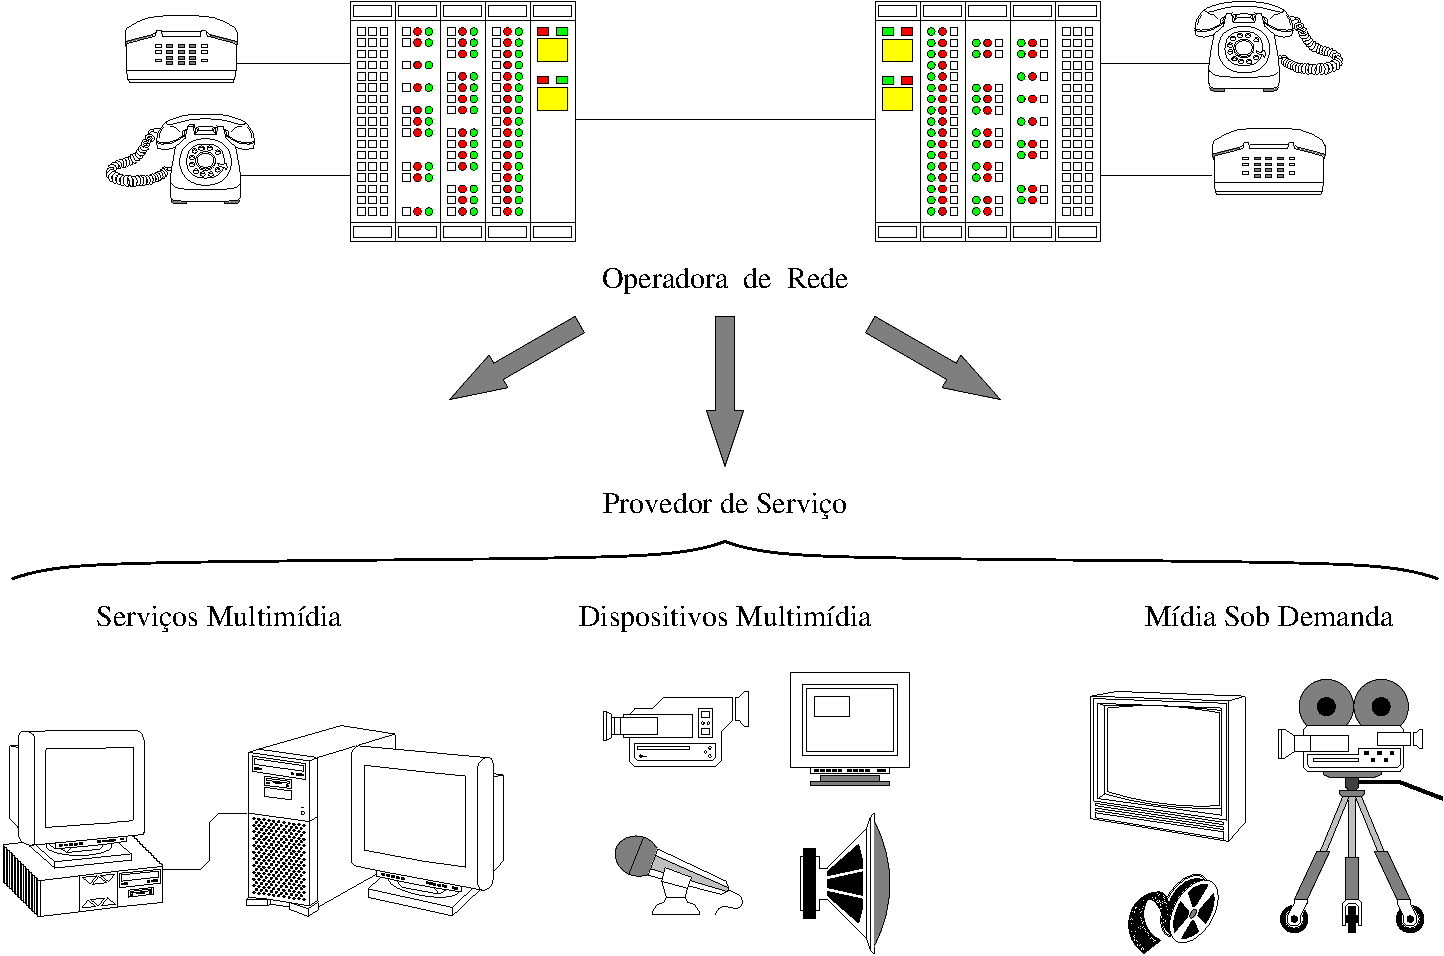
\includegraphics[width=0.55\textwidth]{./CapituloExemplo/figura1}%% Dimensões e localização
\fonte{\citet{Larsson2003}.}%% Fonte
\end{figure}

Figuras em formato GIF, JPEG e BMP podem ser convertidas para o formato \gls{eps} através do aplicativo ``xv''. O ``xv'' não lista o formato \gls{eps} dentre aqueles que é capaz de manipular. Entretanto, selecionando-se o formato \textit{PostScript} e fornecendo-se a extensão \texttt{eps} ao nome do arquivo, o formato \gls{eps} é gerado.

O ambiente \texttt{picture} permite a programação de imagens diretamente no \gls{latex}\index{LaTeX@\latex}, conforme exemplo apresentado na \autoref{fig:figura2}.

\begin{figure}[htb]%% Ambiente figure
\captionsetup{width=8cm}%% Largura da legenda
\caption{Exemplo de figura criada a partir do ambiente \texttt{picture}.}%% Legenda
\label{fig:figura2}%% Rótulo
\setlength{\unitlength}{1cm}%% Unidade de comprimento
\begin{picture}(8,5)(-4,-2.5)%% Ambiente picture
\put(-4,0){\vector(1,0){8}}
\put(3.75,-0.25){$\chi$}
\put(0,-2.5){\vector(0,1){5}}
\multiput(-4,1)(0.4,0){20}{\line(1,0){0.2}}
\multiput(-4,-1)(0.4,0){20}{\line(1,0){0.2}}
\put(0.25,2.25){$\beta \equiv v / c = \tanh \chi$}
\qbezier(0,0)(0.8853,0.8853)(2,0.9640)
\qbezier(0,0)(-0.8853,-0.8853)(-2,-0.9640)
\end{picture}
\fonte{Autoria própria.}%% Fonte
\end{figure}

A \autoref{fig:subfigure} apresenta um exemplo usando o pacote \texttt{subfigure} com legendas usando o pacote \texttt{subcaption}. É  possível referenciar cada uma das sub-figuras, no qual, a sua referência alfabética aparece entre parênteses: \autoref{fig:subfigure_a} e \autoref{fig:subfigure_b}.

\begin{figure}[!ht]
\centering
\caption{Exemplo de Subfigure} 
\label{fig:subfigure}
\begin{subfigure}[t]{.45\textwidth}
	\centering
	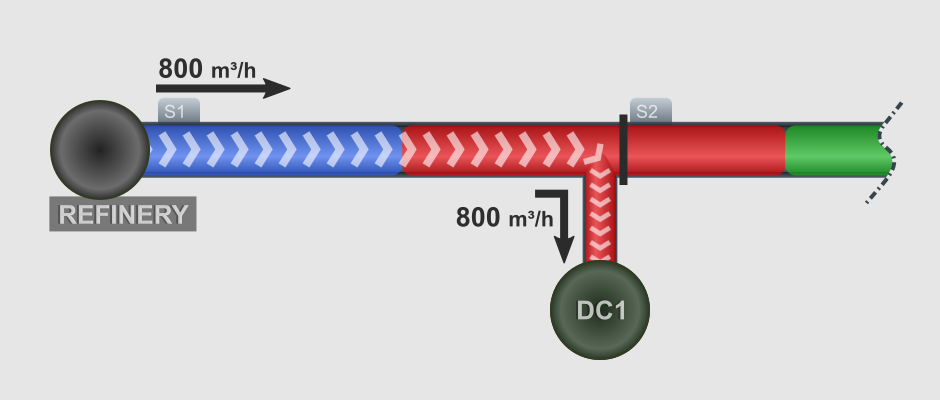
\includegraphics[width=\textwidth]{./CapituloExemplo/subfigure-a.png}
	\caption{Figura A}
	\label{fig:subfigure_a}
\end{subfigure}
\qquad
\begin{subfigure}[t]{.45\textwidth}
	\centering
	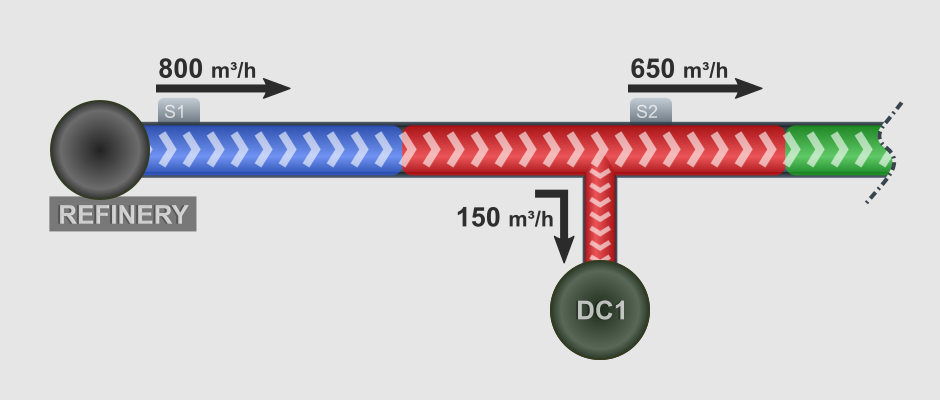
\includegraphics[width=\textwidth]{./CapituloExemplo/subfigure-b.png}  
	\caption{Figura B}
	\label{fig:subfigure_b}
\end{subfigure}
\fonte{\citet{Meira2020}} %citeonline{meira2020}
\end{figure}

%% Título e rótulo de seção (rótulos não devem conter caracteres especiais, acentuados ou cedilha)
\subsection{Fotografias}\label{sec:fotografias}

Um exemplo deste tipo de ilustração é apresentado na \autoref{foto:foto1}.

\begin{photograph}[htb]%% Ambiente photograph
\captionsetup{width=0.6\textwidth}%% Largura da legenda
\caption{Camaleão pantera fotografado por Joel Sartore, National Geographic.}%% Legenda
\label{foto:foto1}%% Rótulo
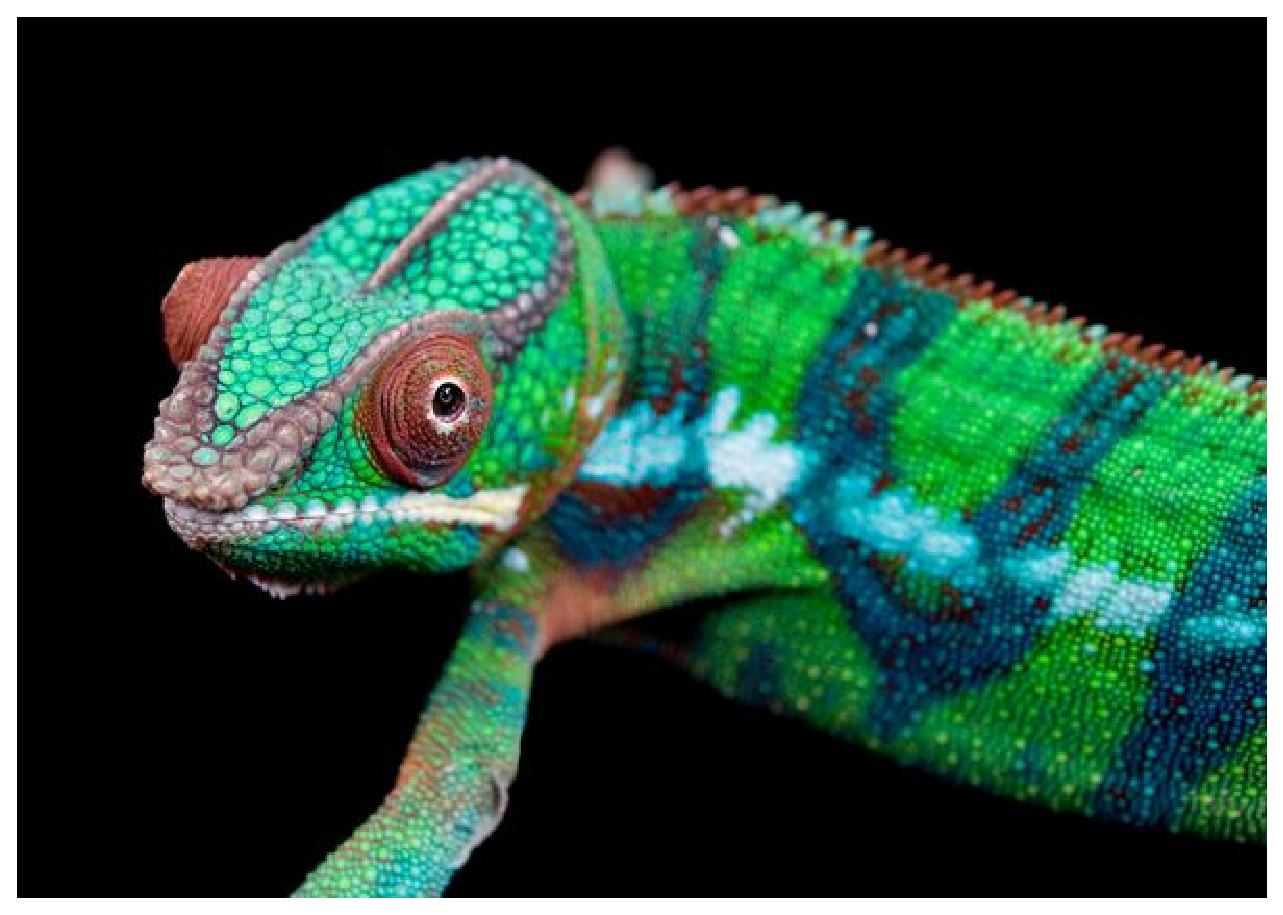
\includegraphics[width=0.6\textwidth]{./CapituloExemplo/foto1}%% Dimensões e localização
\fonte{\citet{Sartore2013}.}%% Fonte
\end{photograph}

Outro exemplo deste tipo de ilustração é apresentado na \autoref{foto:foto2}.

\begin{photograph}[htb]%% Ambiente photograph
\captionsetup{width=0.6\textwidth}%% Largura da legenda
\caption{Fotografia da erupção vulcânica em 1982 do Galungung, Indonésia (com descargas de raios), produzida pelo Serviço Geológico dos Estados Unidos da América.}%% Legenda
\label{foto:foto2}%% Rótulo
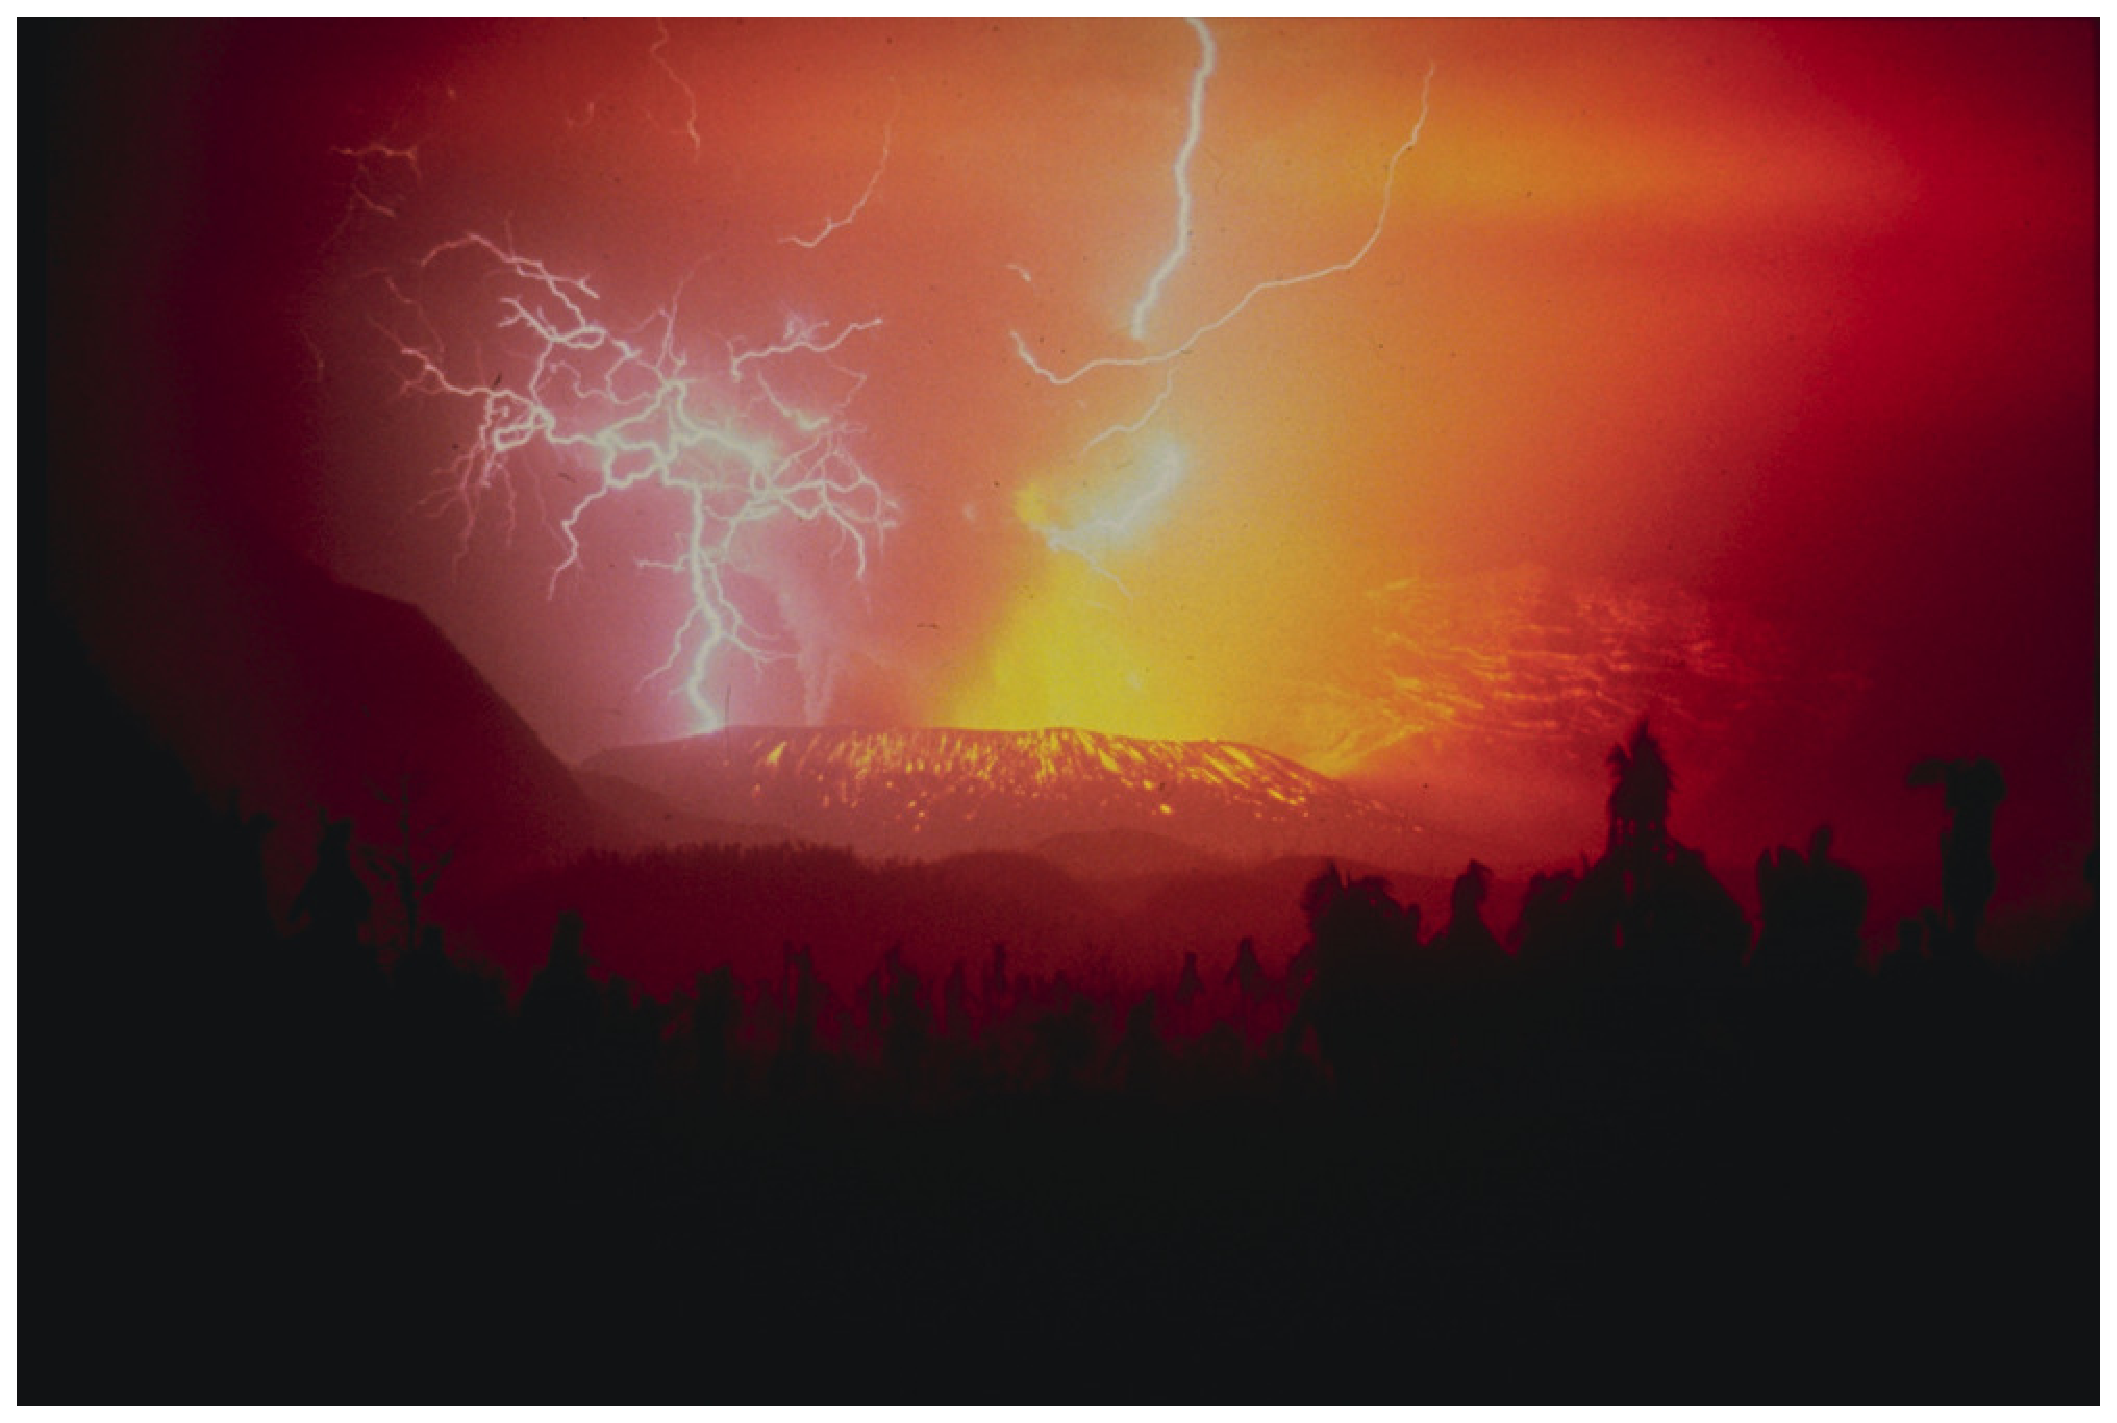
\includegraphics[width=0.6\textwidth]{./CapituloExemplo/foto2}%% Dimensões e localização
\fonte{\citet{Hadian1982}.}%% Fonte
\end{photograph}

%% Título e rótulo de seção (rótulos não devem conter caracteres especiais, acentuados ou cedilha)
\subsection{Gráficos}\label{sec:graficos}

Gráficos são gerados com aplicativos capazes de exportar nos formatos \gls{ps} ou \gls{eps}. A ferramenta ``gnuplot'' é uma das mais utilizadas para a geração de gráficos (\url{http://www.gnuplot.info/}). Uma vez no formato \gls{eps}, gráficos são inseridos no texto tal como figuras (veja \autoref{gra:grafico1}).

\begin{graph}[htb]%% Ambiente graph
\captionsetup{width=0.6\textwidth}%% Largura da legenda
\caption{Exemplo de gráfico produzido em ``gnuplot''.}%% Legenda
\label{gra:grafico1}%% Rótulo
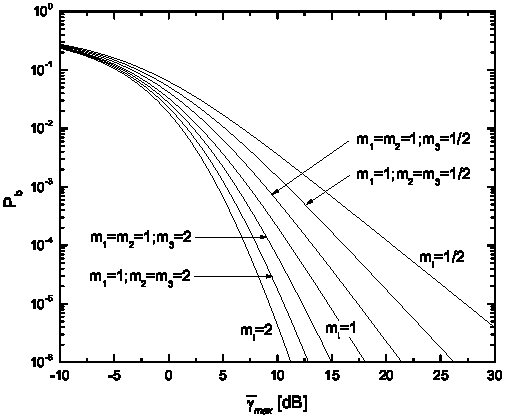
\includegraphics[width=0.6\textwidth]{./CapituloExemplo/grafico1}%% Dimensões e localização
\fonte{\citet{Faina2001}.}%% Fonte
\end{graph}

No \autoref{gra:grafico2} é apresentado um exemplo de gráfico produzido em ``Excel''.

\begin{graph}[htb]%% Ambiente graph
\captionsetup{width=0.6\textwidth}%% Largura da legenda
\caption{Exemplo de gráfico produzido em ``Excel''.}%% Legenda
\label{gra:grafico2}%% Rótulo
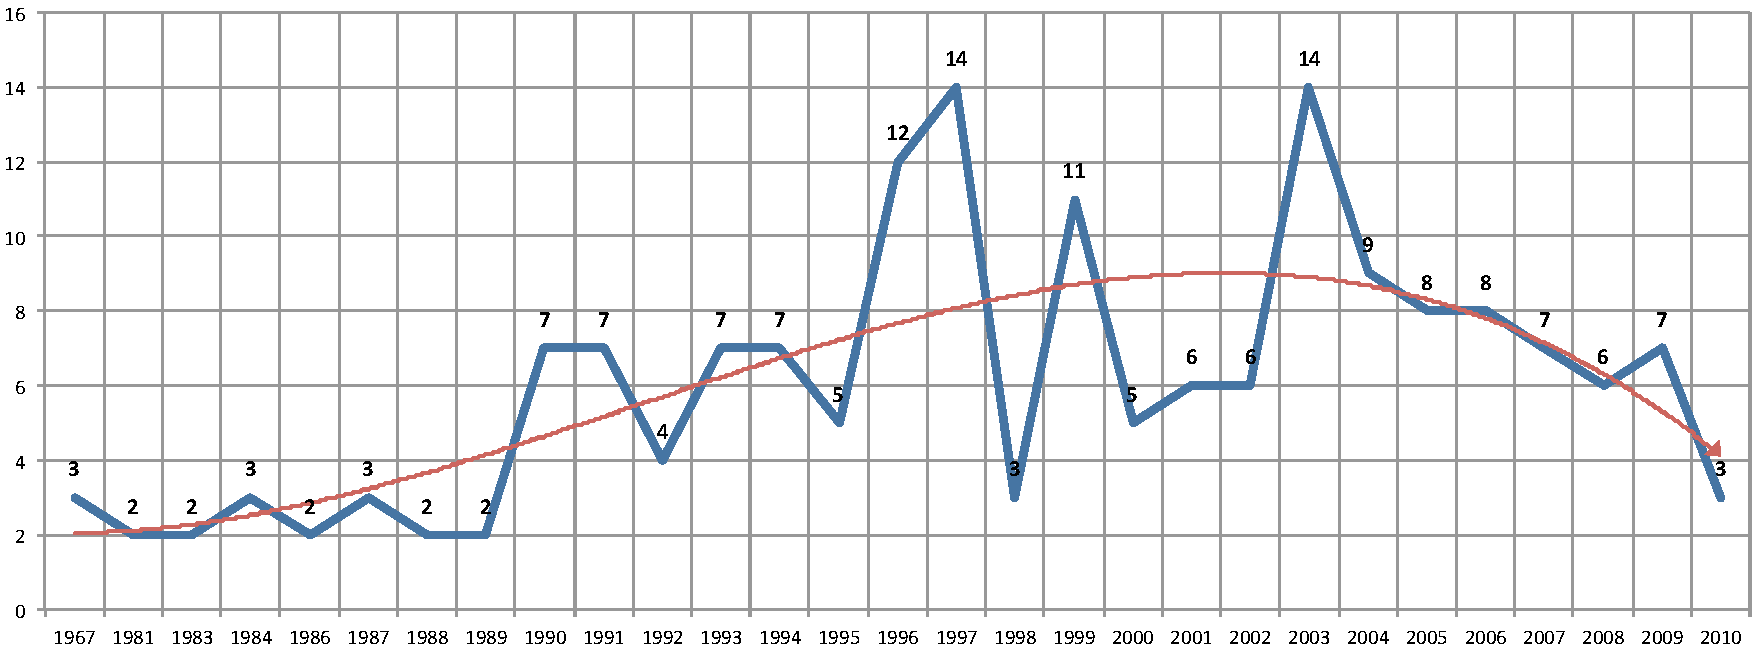
\includegraphics[width=0.6\textwidth]{./CapituloExemplo/grafico2}%% Dimensões e localização
\fonte{\citeonline[p. 24]{Araujo2012}.}%% Fonte
\end{graph}

O ambiente \texttt{minipage} pode ser usado para inserir textos ou outros elementos em quadros com tamanhos e posições controladas, conforme exemplos apresentados no \autoref{gra:minipagegrafico1} e no \autoref{gra:minipagegrafico2}.

\begin{graph}[htb]%% Ambiente graph
\begin{minipage}[t]{0.395\textwidth}%% Ambiente minipage
\centering%% Centralizado
\captionsetup{width=0.85\textwidth}%% Largura da legenda
\caption{Gráfico 1 do ambiente \texttt{minipage}.}%% Legenda
\label{gra:minipagegrafico1}%% Rótulo
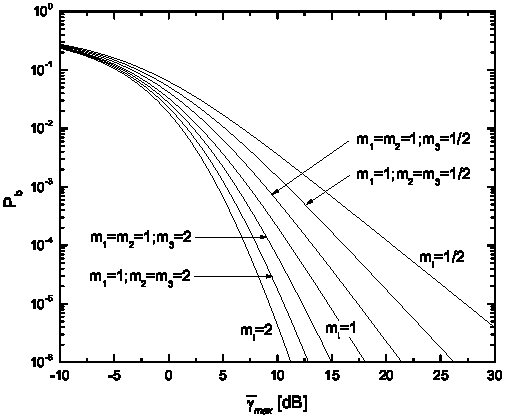
\includegraphics[width=0.85\textwidth]{./CapituloExemplo/grafico1}%% Dimensões e localização
\fonte{\citet{Faina2001}.}%% Fonte
\end{minipage}
\hfill
\begin{minipage}[t]{0.595\textwidth}%% Ambiente minipage
\centering%% Centralizado
\captionsetup{width=0.95\textwidth}%% Largura da legenda
\caption{Gráfico 2 do ambiente \texttt{minipage}.}%% Legenda
\label{gra:minipagegrafico2}%% Rótulo
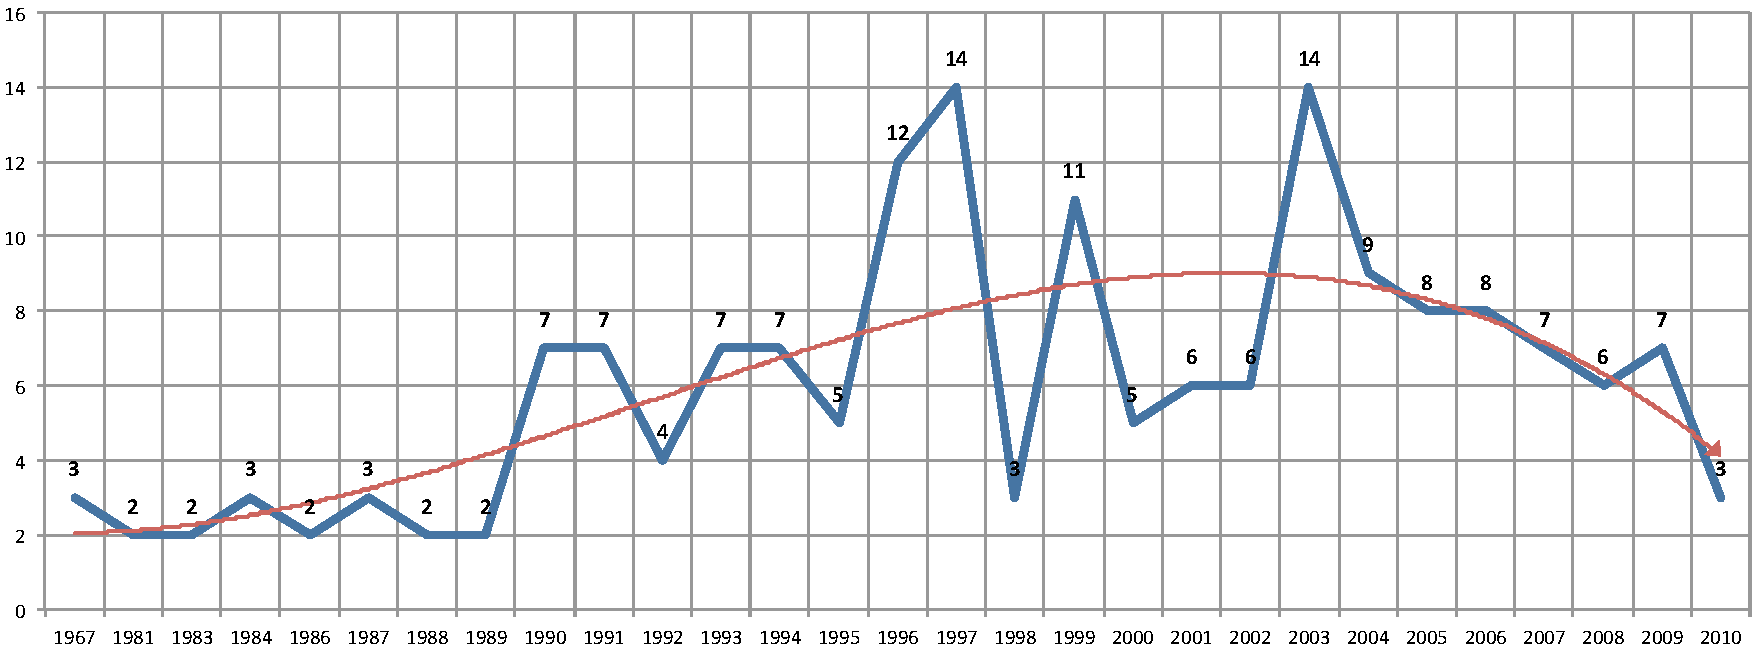
\includegraphics[width=0.95\textwidth]{./CapituloExemplo/grafico2}%% Dimensões e localização
\fonte{\citeonline[p. 24]{Araujo2012}}%% Fonte
\end{minipage}
\label{gra:minipagegraficos}
\end{graph}

%% Título e rótulo de seção (rótulos não devem conter caracteres especiais, acentuados ou cedilha)
\subsection{Quadros}\label{sec:quadros}

Um exemplo deste tipo de ilustração é apresentado no \autoref{quad:quadro1}.

\begin{tabframed}[htb]%% Ambiente tabframed
\captionsetup{width=0.5\textwidth}%% Largura da legenda
\caption{Compostos orgânicos: fórmulas estruturais e principais classes.}%% Legenda
\label{quad:quadro1}%% Rótulo
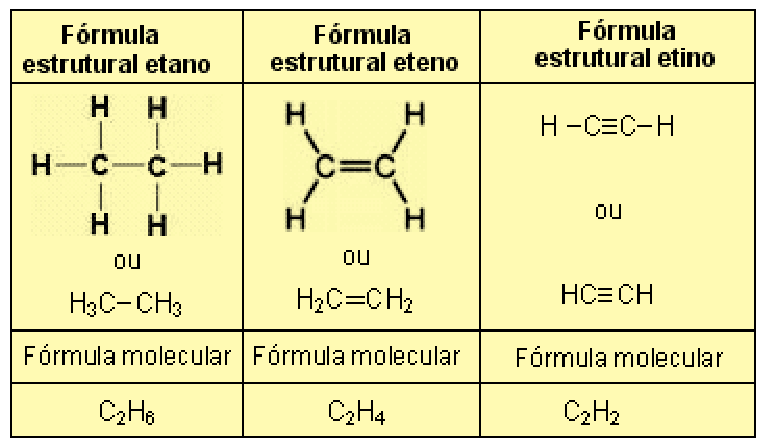
\includegraphics[width=0.5\textwidth]{./CapituloExemplo/quadro1}%% Dimensões e localização
\fonte{\citet{daSilva2009}.}%% Fonte
\end{tabframed}

Outro exemplo deste tipo de ilustração é apresentado no \autoref{quad:quadro2}.

\begin{tabframed}[htb]%% Ambiente tabframed
\captionsetup{width=0.7\textwidth}%% Largura da legenda
\caption{Modelos de maturidade para a gestão da cadeia de suprimentos.}%% Legenda
\label{quad:quadro2}%% Rótulo
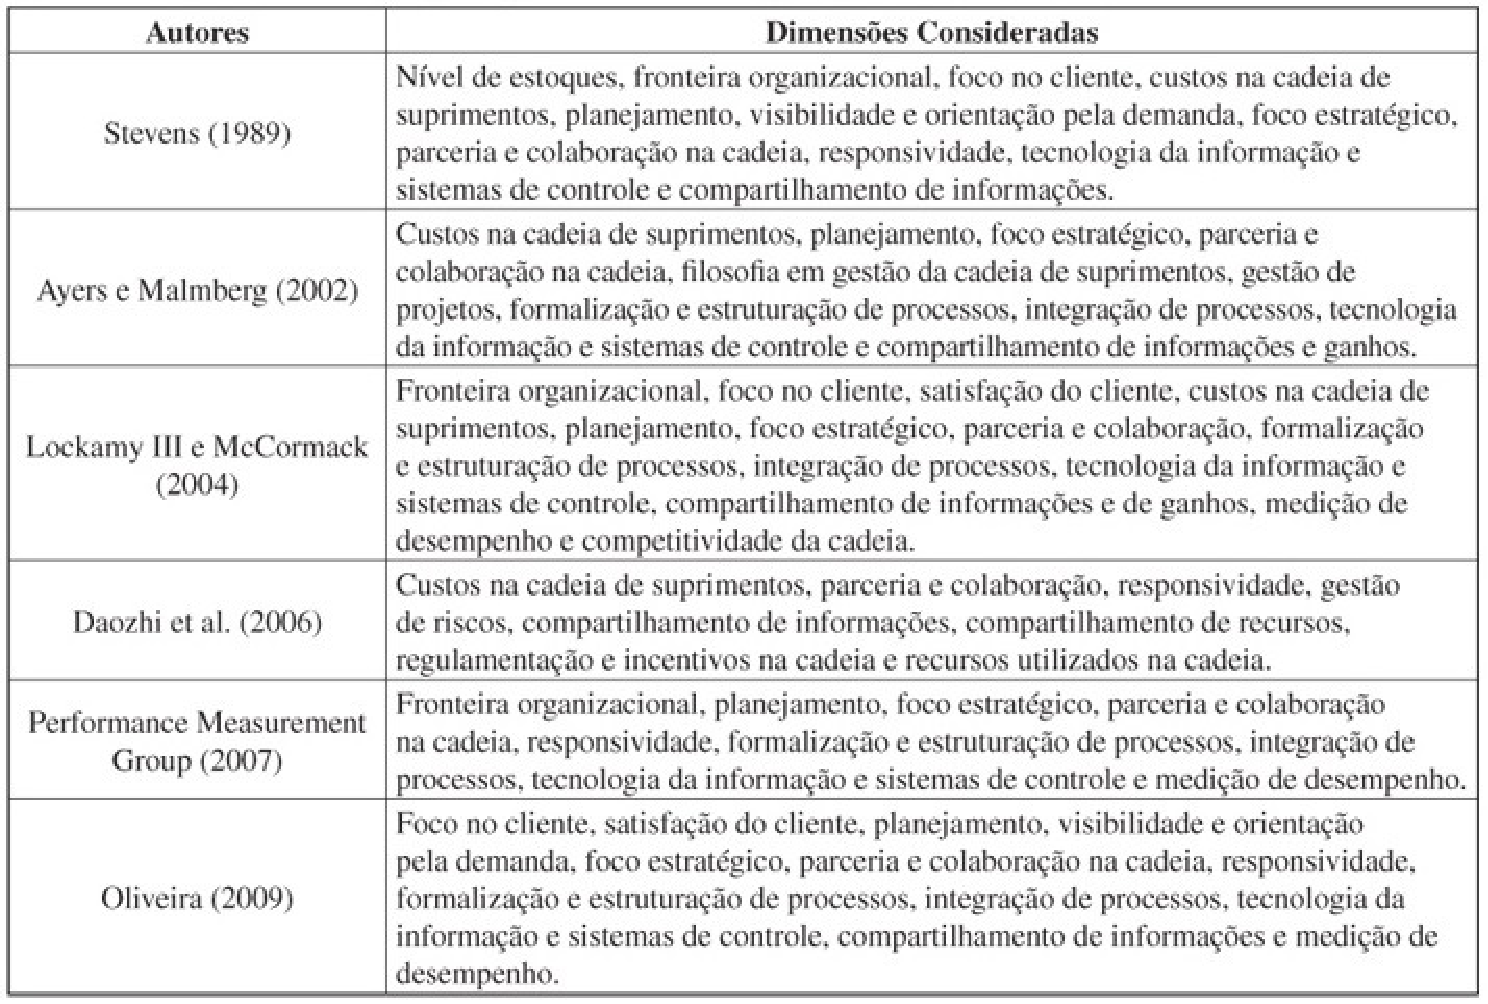
\includegraphics[width=0.7\textwidth]{./CapituloExemplo/quadro2}%% Dimensões e localização
\fonte{\citet{Frederico2012}.}%% Fonte
\end{tabframed}

Os quadros não devem ser chamados de tabelas, uma vez que se diferenciam destas por apresentarem as laterais fechadas e o conteúdo não numérico.

%% Título e rótulo de seção (rótulos não devem conter caracteres especiais, acentuados ou cedilha)
\section{Tabelas}\label{sec:tabelas}

Tabelas são construídas com comandos próprios do \gls{latex}\index{LaTeX@\latex}. Por exemplo, a \autoref{tab:tabela1} foi construída desta forma.

\begin{table}[htb]%% Ambiente table
\caption{Primeiro exemplo de tabela com uma legenda contendo um texto muito longo que pode ocupar mais de uma linha.}%% Legenda
\label{tab:tabela1}%% Rótulo
\begin{tabularx}{\textwidth}{@{\extracolsep{\fill}}llll}%% Ambiente tabularx
\toprule
$\bsym{L}$ & $\bsym{L^2}$ & $\bsym{L^3}$ & $\bsym{L^4}$ \\
\SI{}{[m]} & \SI{}{[m^2]} & \SI{}{[m^3]} & \SI{}{[m^4]} \\ \midrule
1          & 1            & 1            & 1            \\
2          & 4            & 8            & 16           \\
3          & 9            & 27           & 81           \\
4          & 16           & 64           & 256          \\
5          & 25           & 125          & 625          \\ \bottomrule
\end{tabularx}
\fonte{Autoria própria.}%% Fonte
\end{table}

A \autoref{tab:tabela2} é um exemplo de tabela que ocupa mais de uma página e que foi construída pelo \gls{latex}\index{LaTeX@\latex} utilizando o pacote \texttt{longtable}.

\begin{longtable}{@{\extracolsep{\fill}}lll}%% Ambiente longtable
\caption{Possíveis tríplices para grade altamente variável.\label{tab:tabela2}} \\%% Legenda e rótulo
\toprule
\textbf{Tempo (s)} & \textbf{Tríplice escolhida} & \textbf{Outras possíveis tríplices} \\
\midrule
\endfirsthead%% Encerra cabeçalho da primeira página
\caption[]{Possíveis tríplices para grade altamente variável.} \\%% Legenda
\multicolumn{3}{r}{\textbf{(continuação)}} \\
\toprule
\textbf{Tempo (s)} & \textbf{Tríplice escolhida} & \textbf{Outras possíveis tríplices} \\
\midrule
\endhead%% Encerra cabeçalho das demais páginas
\midrule
\multicolumn{3}{r}{\textbf{(continua)}} \\
\endfoot%% Encerra rodapé das demais páginas
\bottomrule
\\[-0.5\linha]
\caption*{\nomefonte: Adaptado de \citet{Smallen2014}.} \\
\endlastfoot%% Encerra rodapé da última página
0      & (1, 11, 13725) & (1, 12, 10980), (1, 13, 8235), (2, 2, 0), (3, 1, 0) \\
2745   & (1, 12, 10980) & (1, 13, 8235), (2, 2, 0), (2, 3, 0), (3, 1, 0)      \\
5490   & (1, 12, 13725) & (2, 2, 2745), (2, 3, 0), (3, 1, 0)                  \\
8235   & (1, 12, 16470) & (1, 13, 13725), (2, 2, 2745), (2, 3, 0), (3, 1, 0)  \\
10980  & (1, 12, 16470) & (1, 13, 13725), (2, 2, 2745), (2, 3, 0), (3, 1, 0)  \\
13725  & (1, 12, 16470) & (1, 13, 13725), (2, 2, 2745), (2, 3, 0), (3, 1, 0)  \\
16470  & (1, 13, 16470) & (2, 2, 2745), (2, 3, 0), (3, 1, 0)                  \\
19215  & (1, 12, 16470) & (1, 13, 13725), (2, 2, 2745), (2, 3, 0), (3, 1, 0)  \\
21960  & (1, 12, 16470) & (1, 13, 13725), (2, 2, 2745), (2, 3, 0), (3, 1, 0)  \\
24705  & (1, 12, 16470) & (1, 13, 13725), (2, 2, 2745), (2, 3, 0), (3, 1, 0)  \\
27450  & (1, 12, 16470) & (1, 13, 13725), (2, 2, 2745), (2, 3, 0), (3, 1, 0)  \\
30195  & (2, 2, 2745)   & (2, 3, 0), (3, 1, 0)                                \\
32940  & (1, 13, 16470) & (2, 2, 2745), (2, 3, 0), (3, 1, 0)                  \\
35685  & (1, 13, 13725) & (2, 2, 2745), (2, 3, 0), (3, 1, 0)                  \\
38430  & (1, 13, 10980) & (2, 2, 2745), (2, 3, 0), (3, 1, 0)                  \\
41175  & (1, 12, 13725) & (1, 13, 10980), (2, 2, 2745), (2, 3, 0), (3, 1, 0)  \\
43920  & (1, 13, 10980) & (2, 2, 2745), (2, 3, 0), (3, 1, 0)                  \\
46665  & (2, 2, 2745)   & (2, 3, 0), (3, 1, 0)                                \\
49410  & (2, 2, 2745)   & (2, 3, 0), (3, 1, 0)                                \\
52155  & (1, 12, 16470) & (1, 13, 13725), (2, 2, 2745), (2, 3, 0), (3, 1, 0)  \\
54900  & (1, 13, 13725) & (2, 2, 2745), (2, 3, 0), (3, 1, 0)                  \\
57645  & (1, 13, 13725) & (2, 2, 2745), (2, 3, 0), (3, 1, 0)                  \\
60390  & (1, 12, 13725) & (2, 2, 2745), (2, 3, 0), (3, 1, 0)                  \\
63135  & (1, 13, 16470) & (2, 2, 2745), (2, 3, 0), (3, 1, 0)                  \\
65880  & (1, 13, 16470) & (2, 2, 2745), (2, 3, 0), (3, 1, 0)                  \\
68625  & (2, 2, 2745)   & (2, 3, 0), (3, 1, 0)                                \\
71370  & (1, 13, 13725) & (2, 2, 2745), (2, 3, 0), (3, 1, 0)                  \\
74115  & (1, 12, 13725) & (2, 2, 2745), (2, 3, 0), (3, 1, 0)                  \\
76860  & (1, 13, 13725) & (2, 2, 2745), (2, 3, 0), (3, 1, 0)                  \\
79605  & (1, 13, 13725) & (2, 2, 2745), (2, 3, 0), (3, 1, 0)                  \\
82350  & (1, 12, 13725) & (2, 2, 2745), (2, 3, 0), (3, 1, 0)                  \\
85095  & (1, 12, 13725) & (1, 13, 10980), (2, 2, 2745), (2, 3, 0), (3, 1, 0)  \\
87840  & (1, 13, 16470) & (2, 2, 2745), (2, 3, 0), (3, 1, 0)                  \\
90585  & (1, 13, 16470) & (2, 2, 2745), (2, 3, 0), (3, 1, 0)                  \\
93330  & (1, 13, 13725) & (2, 2, 2745), (2, 3, 0), (3, 1, 0)                  \\
96075  & (1, 13, 16470) & (2, 2, 2745), (2, 3, 0), (3, 1, 0)                  \\
98820  & (1, 13, 16470) & (2, 2, 2745), (2, 3, 0), (3, 1, 0)                  \\
101565 & (1, 13, 13725) & (2, 2, 2745), (2, 3, 0), (3, 1, 0)                  \\
104310 & (1, 13, 16470) & (2, 2, 2745), (2, 3, 0), (3, 1, 0)                  \\
107055 & (1, 13, 13725) & (2, 2, 2745), (2, 3, 0), (3, 1, 0)                  \\
109800 & (1, 13, 13725) & (2, 2, 2745), (2, 3, 0), (3, 1, 0)                  \\
112545 & (1, 12, 16470) & (1, 13, 13725), (2, 2, 2745), (2, 3, 0), (3, 1, 0)  \\
115290 & (1, 13, 16470) & (2, 2, 2745), (2, 3, 0), (3, 1, 0)                  \\
118035 & (1, 13, 13725) & (2, 2, 2745), (2, 3, 0), (3, 1, 0)                  \\
120780 & (1, 13, 16470) & (2, 2, 2745), (2, 3, 0), (3, 1, 0)                  \\
123525 & (1, 13, 13725) & (2, 2, 2745), (2, 3, 0), (3, 1, 0)                  \\
126270 & (1, 12, 16470) & (1, 13, 13725), (2, 2, 2745), (2, 3, 0), (3, 1, 0)  \\
129015 & (2, 2, 2745)   & (2, 3, 0), (3, 1, 0)                                \\
131760 & (2, 2, 2745)   & (2, 3, 0), (3, 1, 0)                                \\
134505 & (1, 13, 16470) & (2, 2, 2745), (2, 3, 0), (3, 1, 0)                  \\
137250 & (1, 13, 13725) & (2, 2, 2745), (2, 3, 0), (3, 1, 0)                  \\
139995 & (2, 2, 2745)   & (2, 3, 0), (3, 1, 0)                                \\
142740 & (2, 2, 2745)   & (2, 3, 0), (3, 1, 0)                                \\
145485 & (1, 12, 16470) & (1, 13, 13725), (2, 2, 2745), (2, 3, 0), (3, 1, 0)  \\
148230 & (2, 2, 2745)   & (2, 3, 0), (3, 1, 0)                                \\
150975 & (1, 13, 16470) & (2, 2, 2745), (2, 3, 0), (3, 1, 0)                  \\
153720 & (1, 12, 13725) & (2, 2, 2745), (2, 3, 0), (3, 1, 0)                  \\
156465 & (1, 13, 13725) & (2, 2, 2745), (2, 3, 0), (3, 1, 0)                  \\
159210 & (1, 13, 13725) & (2, 2, 2745), (2, 3, 0), (3, 1, 0)                  \\
161955 & (1, 13, 16470) & (2, 2, 2745), (2, 3, 0), (3, 1, 0)                  \\
164700 & (1, 13, 13725) & (2, 2, 2745), (2, 3, 0), (3, 1, 0)                  \\
\end{longtable}

Tabelas criadas em planilhas do ``Excel'' podem ser convertidas em tabelas \gls{latex}\index{LaTeX@\latex} através do suplemento ``Excel-to-LaTeX'', disponível em \url{http://www.ctan.org/pkg/excel2latex}.

%% Título e rótulo de seção (rótulos não devem conter caracteres especiais, acentuados ou cedilha)
\section{Abreviaturas, Siglas e Acrônimos}\label{sec:acronimos}

\gls{latex}\index{LaTeX@\latex} gera automaticamente a lista de abreviaturas, siglas e acrônimos através do pacote \texttt{glossaries}. As abreviaturas, siglas e acrônimos devem ser definidos no arquivo \texttt{entradas-acronimos.tex}, no diretório ``PreTexto'', com os comandos:

\begin{SingleSpacing}%% Ambiente SingleSpacing
\begin{verbatim}
\abreviatura{rótulo}{representação}{definição}
\sigla{rótulo}{representação}{definição}
\acronimo{rótulo}{representação}{definição}
\end{verbatim}
\end{SingleSpacing}

Para que a abreviatura, sigla ou acrônimo seja apresentada em alguma parte do texto do documento use o comando \verb|\gls{rótulo}|, por exemplo, as abreviaturas \gls{art.}, \gls{cap.} e \gls{sec.} foram geradas pelos comandos \verb|\gls{art.}, \gls{cap.} e \gls{sec.}|, respectivamente. Mais detalhes dos comandos do pacote \texttt{glossaries} podem ser encontrados em: \url{http://mirrors.ctan.org/macros/latex/contrib/glossaries/glossaries-user.pdf}.

Outra opção para gerar a lista de abreviaturas, siglas e acrônimos é através da edição manual do arquivo \texttt{lista-acronimos.tex} no diretório ``PreTexto''.

%% Título e rótulo de seção (rótulos não devem conter caracteres especiais, acentuados ou cedilha)
\section{Símbolos}\label{sec:simbolos}

\gls{latex}\index{LaTeX@\latex} gera automaticamente a lista de símbolos através do pacote \texttt{nomencl}. Ao redigir um símbolo pela primeira vez em qualquer parte do texto com o comando \verb|\nomenclature[prefixo]{símbolo}{descrição \nomunit{unidade}}|, é gerada uma entrada para a lista de símbolos. Veja exemplos deste comando no arquivo fonte deste capítulo. Os elementos da lista de símbolos são ordenados a depender da primeira letra atribuída ao prefixo e classificadas em:

\begin{itemize}%% Lista de itens
\item A~-~Letras Latinas.
\item B~-~Letras Gregas.
\item C~-~Sobrescritos.
\item D~-~Subscritos.
\item E~-~Notações.
\item F~-~Índices e Conjuntos
\item G~-~Parâmetros
\item H~-~Variáveis contínuas
\item I~-~Variáveis inteiras
\item J~-~Variáveis binárias
\end{itemize}

Outra opção ao comando \verb|\nomenclature| é o uso dos atalhos:

\begin{SingleSpacing}%% Ambiente SingleSpacing
\begin{verbatim}
\letralatina{prefixo}{símbolo}{descrição}{unidade}
\letragrega{prefixo}{símbolo}{descrição}{unidade}
\sobrescrito{prefixo}{símbolo}{descrição}{unidade}
\subscrito{prefixo}{símbolo}{descrição}{unidade}
\notacao{prefixo}{símbolo}{descrição}{unidade}
\notacaois{símbolo}{descrição}{unidade}
\notacaoparam{símbolo}{descrição}{unidade}
\notacaofloatvar{símbolo}{descrição}{unidade}
\notacaointvar{símbolo}{descrição}{unidade}
\notacaobinvar{símbolo}{descrição}{unidade}
\end{verbatim}
\end{SingleSpacing}

\noindent Neste caso a atribuição da primeira letra do prefixo pode ser desprezada.

%% Letras Latinas [A]
\nomenclature[AA]{$A$}{Área \nomunit{m^2}}%%
\letralatina{L}{L}{Comprimento}{m}%%
\letralatina{R}{R}{Raio}{m}%%
%% Letras Gregas [B]
\nomenclature[Bmu]{$\mu$}{Viscosidade dinâmica \nomunit{kg/(m.s)}}%%
\letragrega{nu}{\nu}{Viscosidade cinemática}{m^2/s}%%
\letragrega{pi}{\pi}{Pi (constante circular)}{rad}%%
\letragrega{rho}{\rho}{Massa específica}{kg/m^3}%%
\letragrega{sigma}{\sigma}{Tensão superficial}{N/m}%%
%% Sobrescritos [C]
\nomenclature[C+]{$+$}{Passo de tempo posterior}%%
\sobrescrito{-}{-}{Passo de tempo anterior}{}%%
\sobrescrito{0}{0}{Valor inicial}{}%%
%% Subscritos [D]
\nomenclature[DG]{$G$}{Fase gasosa}%%
\subscrito{L}{L}{Fase líquida}{}%%
\subscrito{S}{S}{Fase sólida}{}%%
%% Notações [E]
\nomenclature[EPsi_1]{$\overline{\Psi}$}{Média temporal}%%
\notacao{Psi_2}{\langle \Psi \rangle}{Média na seção transversal}{}%%
\notacao{Psi_3}{\langle\langle \Psi \rangle\rangle}{Média na seção transversal ponderada}{}%%
%% Notações [F]
\notacaois{Event_set}{e \in E}{Set of events}{}
\notacaois{Interval_set}{i \in I}{Set of intervals}{}
%% Notações [H]
\notacaoparam{eps}{\varepsilon}{Small constant value}{}
\notacaoparam{lb}{L}{Lower bound value ($L \ll 0$)}{}
%% Notações [I]
\notacaofloatvar{end}{e_{i}}{End of interval $i$}{h}
\notacaofloatvar{start}{s_{i}}{Start of interval $i$}{h}
%% Notações [J]
\notacaointvar{e_i}{\phi_i}{Number of employees set to work during interval $i$}{}
%% Notações [K]
\notacaobinvar{a_i}{a_{i}}{1 if the flow is active during interval $i$; 0 otherwise}{}

Mais detalhes dos comandos do pacote \texttt{nomencl} podem ser encontrados em: \url{http://tug.ctan.org/tex-archive/macros/latex/contrib/nomencl/nomencl.pdf}.

Outra opção para gerar a lista de símbolos é através da edição manual do arquivo \texttt{lista-simbolos.tex} no diretório ``PreTexto''.

%% Título e rótulo de seção (rótulos não devem conter caracteres especiais, acentuados ou cedilha)
\section{Inclusão de Outros Arquivos}\label{sec:inclusao}

É uma boa prática dividir o seu documento em diversos arquivos, e não apenas escrever tudo em um único. Esse recurso foi utilizado neste documento (veja \texttt{utfprct.tex}). Para incluir diferentes arquivos em um arquivo principal, de modo que cada arquivo incluído fique em uma página diferente, utilize o comando:

\begin{SingleSpacing}%% Ambiente SingleSpacing
\begin{verbatim}
\include{documento-a-ser-incluido} %% Sem a extensão .tex
\end{verbatim}
\end{SingleSpacing}

Para incluir documentos sem quebra de páginas, utilize:

\begin{SingleSpacing}%% Ambiente SingleSpacing
\begin{verbatim}
\input{documento-a-ser-incluido}   %% Sem a extensão .tex
\end{verbatim}
\end{SingleSpacing}

%% Título e rótulo de seção (rótulos não devem conter caracteres especiais, acentuados ou cedilha)
\section{Referências Bibliográficas}\label{sec:referencias}

A formatação das referências bibliográficas conforme as regras da \gls{abnt}\index{ABNT} são um dos principais objetivos do \gls{abntex2}\index{abnTeX2@\abnTeX}. Consulte os manuais \citeonline{abnTeX2:2013Cite} e \citeonline{abnTeX2:2013CiteAlf} para obter informações sobre sua utilização.

%% Título e rótulo de seção (rótulos não devem conter caracteres especiais, acentuados ou cedilha)
\subsection{Acentuação de Referências Bibliográficas}\label{sec:acentuacaodereferencias}

Normalmente não há problemas em usar caracteres acentuados em arquivos bibliográficos (extensão \texttt{bib}). Porém, como as regras da \gls{abnt}\index{ABNT} fazem uso quase abusivo da conversão para letras maiúsculas, é preciso observar o modo como se escreve os nomes dos autores e/ou editores. No \autoref{quad:quadro3} você encontra alguns exemplos das conversões mais importantes. A regra geral é sempre usar a acentuação neste modo quando houver conversão para letras maiúsculas.

\begin{tabframed}[htb]%% Ambiente tabframed
\captionsetup{width=0.5\textwidth}%% Largura da legenda
\caption{Conversão de acentuação em arquivos \texttt{bibtex}.}%% Legenda
\label{quad:quadro3}%% Rótulo
\begin{tabular}{|*{2}{p{0.25\textwidth-\columnsep}|}}%% Ambiente tabular
\toprule
\textbf{Acento}   & \textbf{Comando}                       \\ \midrule
{\'a} {\`a} {\~a} & \verb|{\'a}| \verb|{\`a}| \verb|{\~a}| \\ \midrule
{\^e}             & \verb|{\^e}|                           \\ \midrule
{\"u}             & \verb|{\"u}|                           \\ \midrule
{\'\i}            & \verb|{\'\i}|                          \\ \midrule
{\c{c}}           & \verb|{\c{c}}|                         \\ \bottomrule
\end{tabular}
\fonte{Autoria própria.}%% Fonte
\end{tabframed}

%% Título e rótulo de seção (rótulos não devem conter caracteres especiais, acentuados ou cedilha)
\section{Glossário}\label{sec:glossario}

Você pode definir as entradas do glossário no início do texto. Recomenda-se o uso de um arquivo separado a ser inserido ainda no preâmbulo do documento, como por exemplo o arquivo \texttt{entradas-glossario.tex} no diretório ``PosTexto'' do presente documento. Veja orientações sobre inclusão de arquivos na \autoref{sec:inclusao}.

`O \gls{abntex2} é \glsdesc*{abntex2}' é um exemplo de termo definido no glossário e usado no decorrer do texto, bem como:

\begin{citacao}%% Ambiente citacao
Esta frase usa a palavra \gls{componente} e o plural de \glspl{filho}, ambas definidas no glossário como filhas da entrada \gls{pai}. \Gls{equilibrio} exemplifica o uso de um termo no início da frase. O software \gls{abntex2}\index{abnTeX2@\abnTeX} é escrito em \gls{latex}\index{LaTeX@\latex}, que é definido no glossário como `\glsdesc*{latex}'.
\end{citacao}

A frase da citação direta acima foi produzida com:

\begin{SingleSpacing}%% Ambiente SingleSpacing
\begin{verbatim}
Esta frase usa a palavra \gls{componente} e o plural de
\glspl{filho}, ambas definidas no glossário como filhas da
entrada \gls{pai}. \Gls{equilibrio} exemplifica o uso de um
termo no início da frase. O software \gls{abntex2} é
escrito em \gls{latex}, que é definido no glossário como
`\glsdesc*{latex}'.
\end{verbatim}
\end{SingleSpacing}

A impressão efetiva do glossário é dada com:

\begin{SingleSpacing}%% Ambiente SingleSpacing
\begin{verbatim}
\printglossaries
\end{verbatim}
\end{SingleSpacing}

A impressão do glossário incorpora o número das páginas em que as entradas foram citadas. Isso pode ser removido adicionando-se a opção \texttt{nonumberlist} em:

\begin{SingleSpacing}%% Ambiente SingleSpacing
\begin{verbatim}
\usepackage[nonumberlist, style=index]{glossaries}
\end{verbatim}
\end{SingleSpacing}

%% Título e rótulo de seção (rótulos não devem conter caracteres especiais, acentuados ou cedilha)
\section{Apêndices e Anexos}\label{sec:apendiceseanexos}

Apêndices e anexos podem ser inseridos no documento, logo após o glossário, através da inclusão de arquivos, como por exemplo, os arquivos fontes \texttt{apendicea.tex}, \texttt{apendiceb.tex} e  \texttt{anexoa.tex}, presentes no diretório ``PosTexto'' deste projeto, são utilizados para gerar o \autoref{cap:apendicea}, o \autoref{cap:apendiceb} e o \autoref{cap:anexoa}, respectivamente. Veja orientações sobre inclusão de arquivos na \autoref{sec:inclusao}.

%% Título e rótulo de seção (rótulos não devem conter caracteres especiais, acentuados ou cedilha)
\section{Índice Remissivo}\label{sec:indice}

Palavras podem ser indexadas no índice remissivo através do comando \verb|\index{palavra a ser indexada}|. Existem vários exemplos do uso deste comando no arquivo fonte deste capítulo. Por exemplo o comando \verb|\index{Windows}| é utilizado para indexar a palavra Windows\index{Windows} no índice remissivo.

%% Título e rótulo de seção (rótulos não devem conter caracteres especiais, acentuados ou cedilha)
\section{Compilação do Documento \LaTeX}\label{sec:compilar}\index{LaTeX@\latex}

Geralmente os editores \gls{latex}\index{LaTeX@\latex}, como o TeXlipse\index{TeXlipse}\footnote{Disponível em \url{http://texlipse.sourceforge.net/}.}, o Texmaker\index{Texmaker}\footnote{Disponível em \url{http://www.xm1math.net/texmaker/}.}, entre outros, compilam os documentos automaticamente ou após configuração, de modo que você não precisa se preocupar com isto.

No entanto, você pode compilar os documentos \gls{latex}\index{LaTeX@\latex} usando os seguintes comandos, que devem ser digitados no \textit{Prompt} de comandos do Windows\index{Windows} ou no terminal do Mac\index{Mac} ou do Linux\index{Linux}:

\begin{SingleSpacing}%% Ambiente SingleSpacing
\begin{verbatim}
latex <mainfile>.tex
bibtex <mainfile>
latex <mainfile>.tex
latex <mainfile>.tex
dvips <dvips configs> <mainfile>.dvi -o <mainfile>.ps
ps2pdf <mainfile>.ps <mainfile>.pdf
\end{verbatim}
\end{SingleSpacing}

\noindent se todas as figuras no seu documento estão no formato \gls{eps}, ou então, usando os seguintes comandos:

\begin{SingleSpacing}%% Ambiente SingleSpacing
\begin{verbatim}
pdflatex <mainfile>.tex
bibtex <mainfile>
pdflatex <mainfile>.tex
pdflatex <mainfile>.tex
\end{verbatim}
\end{SingleSpacing}

\noindent se todas as figuras no seu documento estão no \gls{pdf}, ou em formatos comuns de imagens (BMP, GIF, JPG ou PNG).

%% Título e rótulo de seção (rótulos não devem conter caracteres especiais, acentuados ou cedilha)
\subsection{Problemas de Compilação}\label{sec:problemas}

O \gls{utfprcttex}\index{UTFPRCTTeX@\utfprcttex} foi configurado e testado para compilar documentos \gls{latex}\index{LaTeX@\latex} sem problemas, mas por se tratar de uma linguagem de programação (para editoração) está sujeita à \textit{bugs} como qualquer outra linguagem. Além disto, o \gls{utfprcttex}\index{UTFPRCTTeX@\utfprcttex} é baseado em outras classes de documento e também utiliza uma quantidade considerável de pacotes que podem ter incompatibilidades. Portanto, alguns cuidados devem ser tomados quando se trabalha com \gls{latex}\index{LaTeX@\latex}, principalmente para novos usuários:

\begin{itemize}%% Lista de itens
\item Os comandos devem ser corretamente finalizados, ou seja, deve-se verificar a abertura e fechamento dos colchetes e chaves: \verb|\comando[opções]{argumentos}|. Alguns comandos não necessitam disto, por exemplo \verb|\comando|, mas as vezes torna-se necessário colocar uma barra invertida, \verb|\|, ou chaves, \verb|{}|, após o comando para gerar um espaço com o texto na sequência: \verb|\comando\ texto na sequência do comando| ou \verb|\comando{} texto na sequência do comando|.
\item Os ambientes devem ser corretamente finalizados, ou seja, deve-se verificar a abertura e fechamento dos ambientes: \verb|\begin{ambiente} ... \end{ambiente}|.
\item Os caracteres especiais devem ser precedidos de barra invertida quando se deseja imprimí-los no texto: \verb|\$ \& \% \# \_ \{ \}| resulta em \$ \& \% \# \_ \{ \}. Do contrário, não serão impressos e executarão comandos específicos do \gls{latex}\index{LaTeX@\latex}.
\item Os textos copiados de outros arquivos (\texttt{*.doc}, \texttt{*.html}, \texttt{*.pdf}, etc.) para os arquivos fonte do \gls{latex}\index{LaTeX@\latex} (\texttt{*.tex}, \texttt{*.bib}, etc.) devem ter a mesma codificação de caracteres (\texttt{UTF8}). Do contrário, alguns caracteres não serão devidamente impressos ou causarão erro, por exemplo, o hífen e os caracteres acentuados.
\item Os nomes de arquivos carregados no modelo (arquivos fontes, figuras, etc.) não devem conter caracteres especiais ou acentuados: \verb|capitulo1.tex| ao invés de \verb|capitulo_1.tex|. Esta regra também se aplica aos rótulos: \verb|\label{cap:capitulo1}| ao invés de \verb|\label{cap:capitulo_1}|.
\end{itemize}

Outras dicas de uso dos comandos do \gls{latex}\index{LaTeX@\latex} podem ser encontradas em diversos materiais de referência disponíveis na internet, por exemplo: \url{http://en.wikibooks.org/wiki/LaTeX}, \url{https://www.overleaf.com/learn}, entre outros.
%% Comente para remover este item


%%%%%%%%%%%%%%%%%%%%%%%%%%%%%%%%%%%%%%%%%%%%%%%
%%%%%%%%%%%%%%%%%%%%%%%%%%%%%%%%%%%%%%%%%%%%%%%
%% Formatação de páginas de elementos pós-textuais
%%
\postextual%% Não comente esta linha


%%%%%%%%%%%%%%%%%%%%%%%%%%%%%%%%%%%%%%%%%%%%%%%
%% Arquivos de referências
%%
\arquivosdereferencias{%% Arquivos bibtex sem a extensão .bib e separados por vírgula - Não comente esta linha
  ./PosTexto/exemplos-referencias,%% Arquivo de referências - Comente para remover este item (chktex 26 supress warn.)
  ./PosTexto/referencias%% Arquivo de referências - Comente para remover este item (chktex 26 - supress warn.)
}%% Não comente esta linha
%%%%%%%%%%%%%%%%%%%%%%%%%%%%%%%%%%%%%%%%%%%%%%%


%%%%%%%%%%%%%%%%%%%%%%%%%%%%%%%%%%%%%%%%%%%%%%%
%% Glossário
%%
\incluirglossario%% Comente para remover este item
%%%%%%%%%%%%%%%%%%%%%%%%%%%%%%%%%%%%%%%%%%%%%%%


%%%%%%%%%%%%%%%%%%%%%%%%%%%%%%%%%%%%%%%%%%%%%%%
%% Arquivos de apêndices
%%
\begin{arquivosdeapendices}%% Os arquivos de apêndices devem se incluídos neste ambiente - Não comente esta linha
  \partapendices%% Página de início dos apêndices - Comente para remover este item
  %%%% APÊNDICE A
%%
%% Texto ou documento elaborado pelo autor, a fim de complementar sua argumentação, sem prejuízo da unidade nuclear do trabalho.

%% Título e rótulo de apêndice (rótulos não devem conter caracteres especiais, acentuados ou cedilha)
\chapter{Título do Apêndice A com um Texto Muito Longo que Pode Ocupar Mais de uma Linha}\label{cap:apendicea}

Quando houver necessidade pode-se apresentar como apêndice documento(s) auxiliar(es) e/ou complementar(es) como: legislação, estatutos, gráficos, tabelas, etc. Os apêndices são enumerados com letras maiúsculas: \autoref{cap:apendicea}, \autoref{cap:apendiceb}, etc.

No \latex\ apêndices são editados como capítulos. O comando \verb|\appendix| faz com que todos os capítulos seguintes sejam considerados apêndices.

Apêndices complementam o texto principal da tese com informações para leitores com especial interesse no tema, devendo ser considerados leitura opcional, ou seja, o entendimento do texto principal da tese não deve exigir a leitura atenta dos apêndices.

Apêndices usualmente contemplam provas de teoremas, deduções de fórmulas matemáticas, diagramas esquemáticos, gráficos e trechos de código. Quanto a este último, código extenso não deve fazer parte da tese, mesmo como apêndice. O ideal é disponibilizar o código na Internet para os interessados em examiná-lo ou utilizá-lo.

%% Título e rótulo de seção (rótulos não devem conter caracteres especiais, acentuados ou cedilha)
%\section{Título da Seção Secundária do Apêndice B}\label{sec:secaoapendicea}

%Exemplo de seção secundária em apêndice (\autoref{sec:secaoapendicea} do \autoref{cap:apendicea}).

%% Título e rótulo de seção (rótulos não devem conter caracteres especiais, acentuados ou cedilha)
%\subsection{Título da Seção Terciária do Apêndice B}\label{subsec:subsecaoapendicea}

%Exemplo de seção terciária em apêndice (\autoref{subsec:subsecaoapendicea} do \autoref{cap:apendicea}).

%% Título e rótulo de seção (rótulos não devem conter caracteres especiais, acentuados ou cedilha)
%\subsubsection{Título da seção quaternária do Apêndice B}\label{subsubsec:subsubsecaoapendicea}

%Exemplo de seção quaternária em apêndice (\autoref{subsubsec:subsubsecaoapendicea} do \autoref{cap:apendicea}).

%% Título e rótulo de seção (rótulos não devem conter caracteres especiais, acentuados ou cedilha)
%\paragraph{Título da seção quinária do Apêndice B}\label{para:paragraphapendicea}

%Exemplo de seção quinária em apêndice (\autoref{para:paragraphapendicea} do \autoref{cap:apendicea}).
%% Apêndice - Comente para remover este item
  %%%% APÊNDICE B
%%
%% Texto ou documento elaborado pelo autor, a fim de complementar sua argumentação, sem prejuízo da unidade nuclear do trabalho.

%% Título e rótulo de apêndice (rótulos não devem conter caracteres especiais, acentuados ou cedilha)
\chapter{Orçamentos dos Materiais para Montagem da Bancada Experimental}\label{cap:apendiceb}

\begin{table}[htb]%% Ambiente table
\caption{Orçamento dos materiais n.\textsuperscript{o} 1.}%% Legenda
\label{tab:tab3}%% Rótulo
\begin{tabularx}{\textwidth}{@{\extracolsep{\fill}}lrrr}%% Ambiente tabularx
\toprule
Material              & \multicolumn{1}{c}{Valor (R\$)} & \multicolumn{1}{c}{Quantidade}  & \multicolumn{1}{c}{Total (R\$)} \\ \midrule
Bomba centrífuga      & 2500,00                         & 01                              & 2500,00                         \\
Compressor rotativo   & 3000,00                         & 01                              & 3000,00                         \\
Manômetro diferencial & 450,00                          & 02                              & 900,00                          \\
Termopar              & 370,00                          & 02                              & 740,00                          \\
Válvula de esfera     & 43,00                           & 02                              & 86,00                           \\
Tubulação de PVC      & 10,00                           & 05                              & 50,00                           \\
Conexão de PVC        & 5,00                            & 10                              & 50,00                           \\ \midrule
                      &                                 & \multicolumn{1}{r}{Total (R\$)} & 7326,00                         \\ \bottomrule
\end{tabularx}
\fonte{}%% Fonte
\end{table}

\begin{table}[htb]%% Ambiente table
\caption{Orçamento dos materiais n.\textsuperscript{o} 2.}%% Legenda
\label{tab:tab4}%% Rótulo
\begin{tabularx}{\textwidth}{@{\extracolsep{\fill}}lrrr}%% Ambiente tabularx
\toprule
Material              & \multicolumn{1}{c}{Valor (R\$)} & \multicolumn{1}{c}{Quantidade}  & \multicolumn{1}{c}{Total (R\$)} \\ \midrule
Bomba centrífuga      & 2700,00                         & 01                              & 2700,00                         \\
Compressor rotativo   & 2950,00                         & 01                              & 2950,00                         \\
Manômetro diferencial & 515,00                          & 02                              & 1030,00                         \\
Termopar              & 350,00                          & 02                              & 700,00                          \\
Válvula de esfera     & 40,00                           & 02                              & 80,00                           \\
Tubulação de PVC      & 8,00                            & 05                              & 40,00                           \\
Conexão de PVC        & 6,00                            & 10                              & 60,00                           \\ \midrule
                      &                                 & \multicolumn{1}{r}{Total (R\$)} & 7560,00                         \\ \bottomrule
\end{tabularx}
\fonte{}%% Fonte
\end{table}

\begin{table}[htb]%% Ambiente table
\caption{Orçamento dos materiais n.\textsuperscript{o} 3.}%% Legenda
\label{tab:tab5}%% Rótulo
\begin{tabularx}{\textwidth}{@{\extracolsep{\fill}}lrrr}%% Ambiente tabularx
\toprule
Material              & \multicolumn{1}{c}{Valor (R\$)} & \multicolumn{1}{c}{Quantidade}  & \multicolumn{1}{c}{Total (R\$)} \\ \midrule
Bomba centrífuga      & 2600,00                         & 01                              & 2600,00                         \\
Compressor rotativo   & 3100,00                         & 01                              & 3100,00                         \\
Manômetro diferencial & 500,00                          & 02                              & 1000,00                         \\
Termopar              & 400,00                          & 02                              & 800,00                          \\
Válvula de esfera     & 45,00                           & 02                              & 90,00                           \\
Tubulação de PVC      & 12,00                           & 05                              & 60,00                           \\
Conexão de PVC        & 5,00                            & 10                              & 50,00                           \\ \midrule
                      &                                 & \multicolumn{1}{r}{Total (R\$)} & 7700,00                         \\ \bottomrule
\end{tabularx}
\fonte{}%% Fonte
\end{table}
%% Apêndice - Comente para remover este item
\end{arquivosdeapendices}%% Não comente esta linha
%%%%%%%%%%%%%%%%%%%%%%%%%%%%%%%%%%%%%%%%%%%%%%%


%%%%%%%%%%%%%%%%%%%%%%%%%%%%%%%%%%%%%%%%%%%%%%%
%% Arquivos de anexos
%%
\begin{arquivosdeanexos}%% Os arquivos de anexos devem se incluídos neste ambiente - Não comente esta linha  
  \partanexos%% Página de início dos anexos - Comente para remover este item (ver Bug0001)
  %%%% ANEXO A
%%
%% Texto ou documento não elaborado pelo autor, que serve de fundamentação, comprovação e ilustração.

%% Título e rótulo de anexo (rótulos não devem conter caracteres especiais, acentuados ou cedilha)
\anexos
%% Anexo - Comente para remover este item
%  %%%%% ANEXO B
%%
%% Texto ou documento não elaborado pelo autor, que serve de fundamentação, comprovação e ilustração.

%% Título e rótulo de anexo (rótulos não devem conter caracteres especiais, acentuados ou cedilha)



%% Anexo - Comente para remover este item
\end{arquivosdeanexos}%% Não comente esta linha
%%%%%%%%%%%%%%%%%%%%%%%%%%%%%%%%%%%%%%%%%%%%%%%


%%%%%%%%%%%%%%%%%%%%%%%%%%%%%%%%%%%%%%%%%%%%%%%
%% Índice
%%
\incluirindice%% Comente para remover este item
%%%%%%%%%%%%%%%%%%%%%%%%%%%%%%%%%%%%%%%%%%%%%%%

%% Fim do documento
\end{document}%% Não comente esta linha
%%%%%%%%%%%%%%%%%%%%%%%%%%%%%%%%%%%%%%%%%%%%%%%